\documentclass[11pt]{report}

\usepackage[margin=1in]{geometry}
\usepackage{amsmath, amssymb, amsthm}
\usepackage{physics}
\usepackage{graphicx}
\usepackage{tikz}
\usepackage{hyperref}
\usepackage{xcolor}
\usepackage{enumitem}

\hypersetup{
    colorlinks=true,
    linkcolor=blue,
    urlcolor=blue
}

\newcommand{\vbf}[1]{\vec{\mathbf{#1}}}
\newcommand{\nhat}{\hat{n}}

\title{E\&M Lecture Notes \\ \large Part 3: Units 9--14}
\author{}
\date{}

\begin{document}
\maketitle
\tableofcontents
\newpage

%==============================================================
% Unit 9: Faraday's Law of Induction
%==============================================================
\chapter{Faraday's Law of Induction}

\section{Faraday's Law of Induction}

An EMF, $\mathcal{E}$, will be induced in a circuit equal to the negative rate of change of magnetic flux through the circuit:
\begin{equation}
\boxed{\mathcal{E} = -\frac{d\Phi_B}{dt}, \qquad \Phi_B = \int \vbf{B} \cdot \nhat \, dA}
\end{equation}

If the circuit is a coil of $N$ turns, then
\begin{equation}
\mathcal{E} = -N \frac{d\Phi_B}{dt} = -\frac{d}{dt}(N\Phi_B), \qquad N\Phi_B \equiv \text{flux linkage}
\end{equation}

\subsection*{Example: Magnet Pushed into a Coil}

Consider a bar magnet (with N pole facing left toward a coil) being pushed into a coil connected to an ammeter. Pushing the magnet into the coil changes the flux $\Phi_B$ through the coil, and induces a current $i$. \emph{What is the direction of $i$?}

\begin{figure}[h]
  \centering
  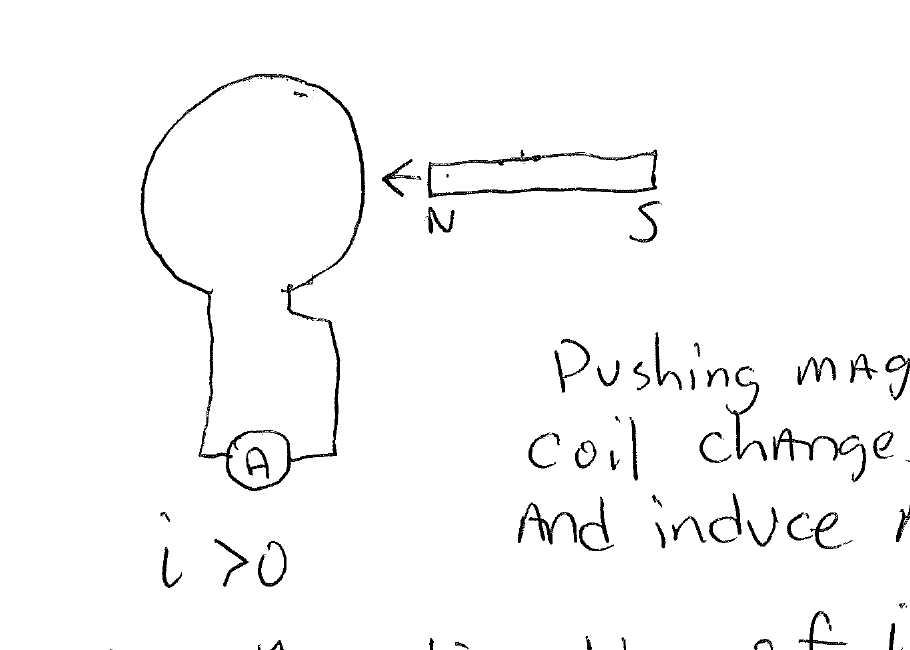
\includegraphics[width=0.45\textwidth,keepaspectratio]{figures/inline/u9_magnet_coil.png}
  \caption*{Magnet pushed into a coil; ammeter reads induced current $i$.}
\end{figure}


\subsection*{Lenz's Law}

\textbf{Lenz's Law:} \emph{The induced current will be in the direction that opposes the changing flux in the circuit.}

\subsubsection*{Two ways to think about Lenz's Law}

\textbf{1) Magnetic dipole picture:} The induced current produces a magnetic dipole moment that effectively makes the coil look like a magnet. When a N-pole is pushed in from the left, the side of the coil facing the incoming magnet becomes a N-pole as well, so the two N-poles \emph{repel} each other (resisting the motion of the magnet into the loop).

\begin{figure}[h]
  \centering
  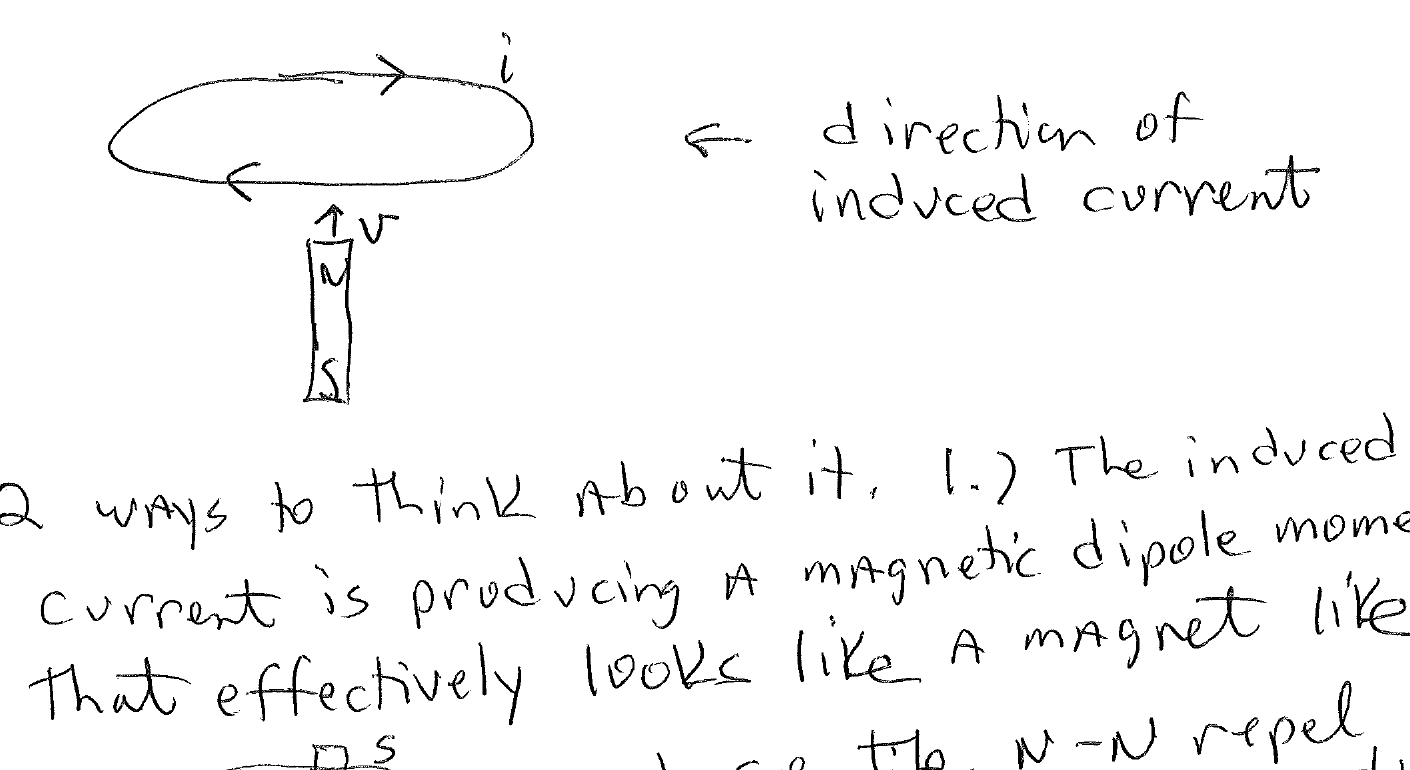
\includegraphics[width=0.7\textwidth,keepaspectratio]{figures/inline/u9_lenz_dipole.png}
  \caption*{Induced current produces a magnetic dipole that repels the incoming N-pole.}
\end{figure}


\textbf{2) Flux cancellation picture:} The induced current produces a B-field inside the loop that points opposite to the magnet's increasing field, thus reducing the change in flux penetrating the loop.

\subsubsection*{Pulling the Magnet Away}

If you pull the magnet away (with N-pole toward the coil moving away), the flux through the loop is now \emph{decreasing}. By Lenz's law, the induced current reverses direction:
\begin{itemize}
    \item The induced current's magnetic dipole now \emph{attracts} the magnet (S-pole faces the receding N-pole).
    \item The induced B-field \emph{adds to} the flux in the loop (to help it persist).

\begin{figure}[h]
  \centering
  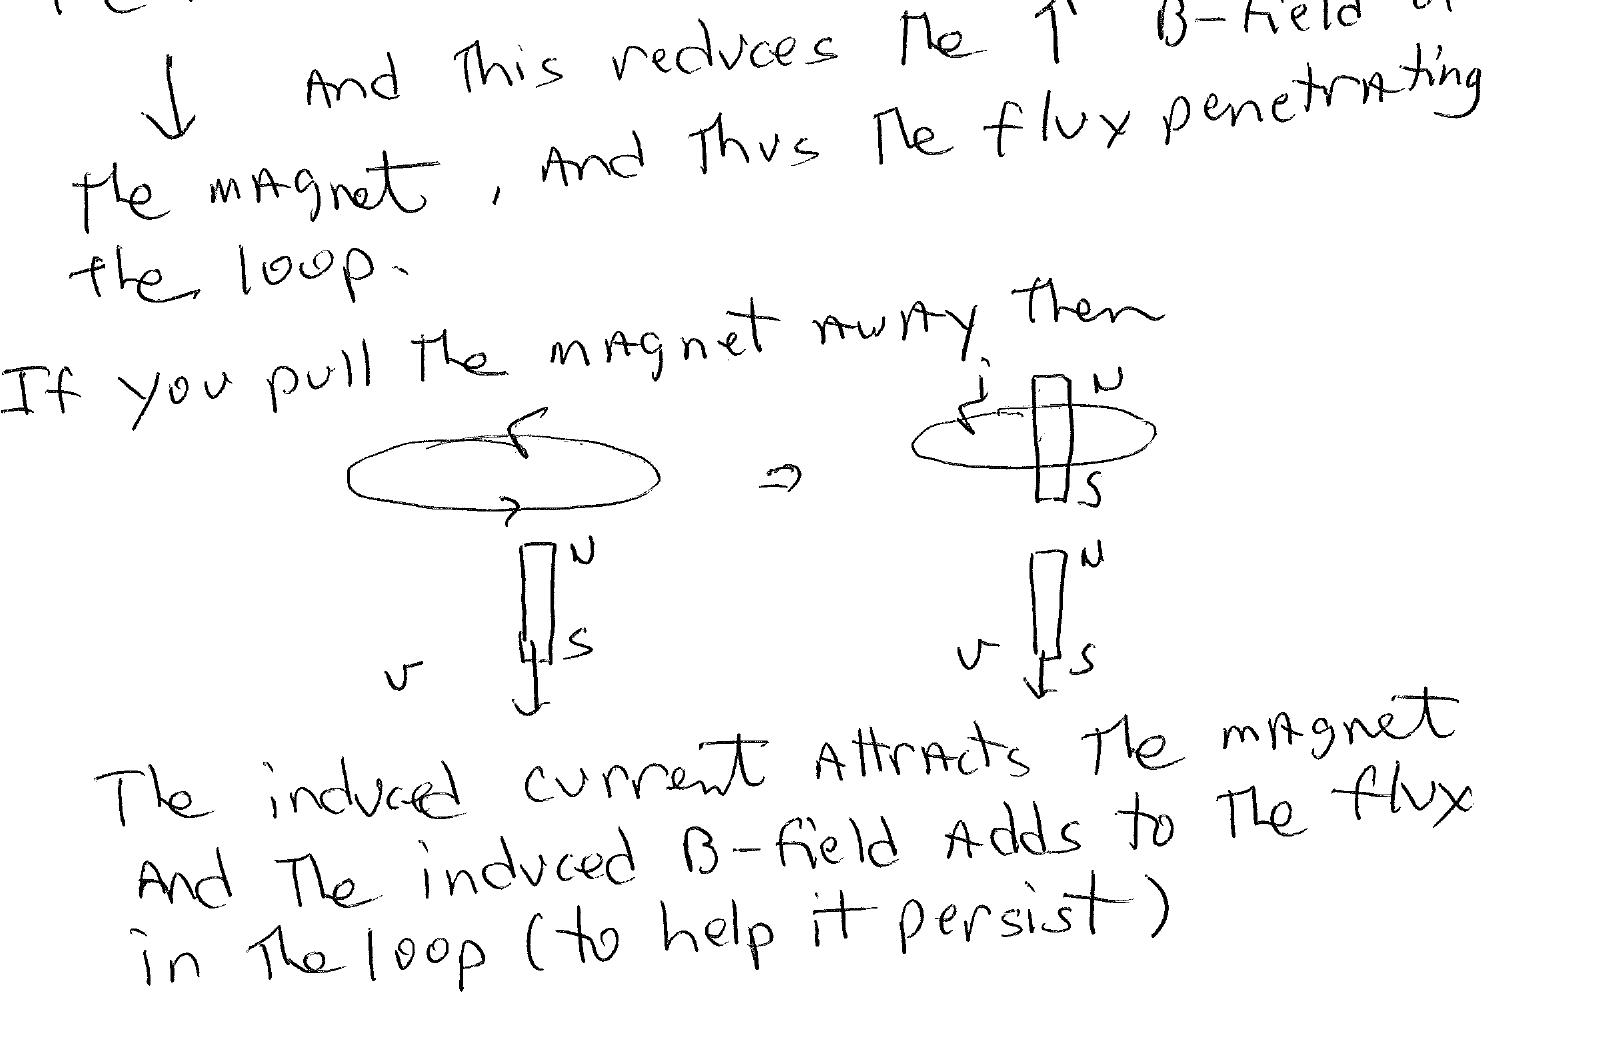
\includegraphics[width=0.8\textwidth,keepaspectratio]{figures/inline/u9_lenz_pull_away.png}
  \caption*{Pulling the magnet away: induced current reverses; loop's S-pole faces the receding N-pole.}
\end{figure}

\end{itemize}

In both cases, the induced effect opposes the \emph{change}, not the flux itself.

\section{Quantitative Induction: Loop in a Uniform B-field}

Consider a rectangular wire loop being pulled out of a uniform magnetic field $\vbf{B}$ (pointing into the page) at speed $v$ by an external force $\vbf{F}_h$ (the ``hand'').

\begin{figure}[h]
  \centering
  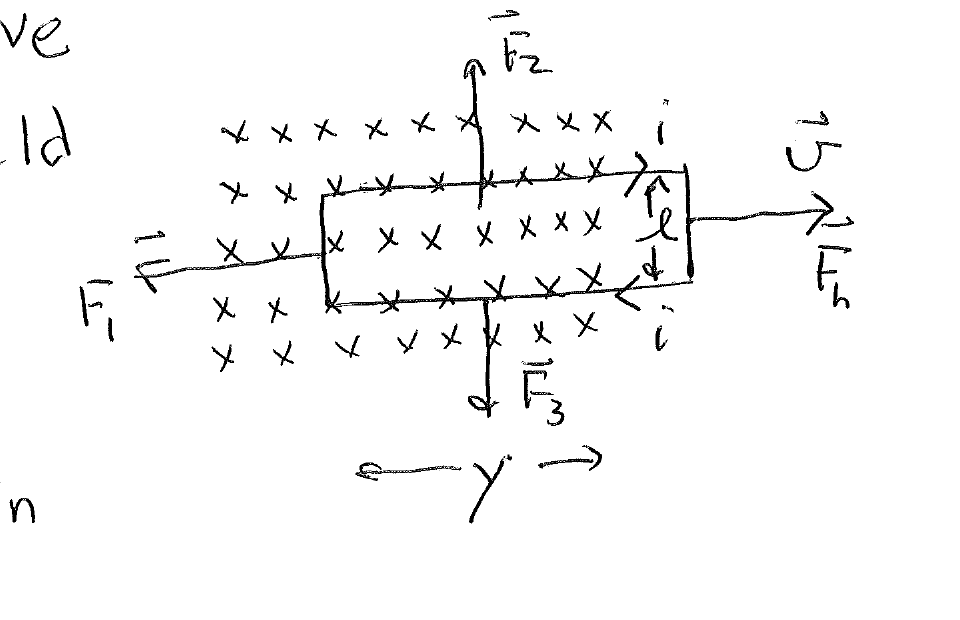
\includegraphics[width=0.55\textwidth,keepaspectratio]{figures/inline/u9_loop_in_B.png}
  \caption*{Loop being pulled out of a uniform B-field (into page) at speed $v$ by force $\vbf{F}_h$.}
\end{figure}


\textbf{Definitions:}
\begin{itemize}
    \item $y = $ length of loop currently inside the B-field
    \item $\ell = $ width of loop (perpendicular to motion)
    \item $\vbf{F}_h = $ force pulling wire loop out of B-field at speed $v$
    \item $i = $ induced current in loop
    \item $R = $ resistance of loop
\end{itemize}

\subsection*{Computing the Induced EMF}

The flux in the loop is
\begin{equation}
\Phi_B = \int \vbf{B} \cdot \nhat \, dA = B\ell y
\end{equation}

Taking the time derivative (as the loop is pulled out, $y$ decreases; we track magnitudes here):
\begin{equation}
\frac{d\Phi_B}{dt} = B\ell \frac{dy}{dt} = B\ell v
\end{equation}

So the induced EMF is
\begin{equation}
-\frac{d\Phi_B}{dt} = \mathcal{E} = B\ell v
\end{equation}

(The minus sign just reminds us to set the current direction by Lenz's Law.)

For loop resistance $R$, the induced current is
\begin{equation}
\boxed{i = \frac{\mathcal{E}}{R} = \frac{B\ell v}{R}}
\end{equation}

The direction of current shown adds flux as it is being reduced by motion out of the B-field --- consistent with Lenz's Law.

\subsection*{Analysis of Forces}

Three pieces of the loop carry current in the B-field. Using $\vbf{F} = i\vbf{L} \times \vbf{B}$ and the right-hand rule (RHR):
\begin{align}
\vbf{F}_2 &= i\vbf{y} \times \vbf{B} = iyB \quad &&\text{(upward)} \\
\vbf{F}_3 &= i\vbf{y} \times \vbf{B} = iyB \quad &&\text{(downward)} \\
\vbf{F}_2 + \vbf{F}_3 &= 0
\end{align}

The vertical forces on the top and bottom segments cancel. For the left vertical segment (still in the field):
\begin{equation}
\vbf{F}_1 = -i\ell B \,\hat{y}
\end{equation}

This force opposes the motion of the loop. The hand must pull with
\begin{equation}
\vbf{F}_h = +i\ell B \,\hat{y}
\end{equation}

Because $\vbf{F}_y = \vbf{F}_1 + \vbf{F}_h = 0 \implies a_y = 0 \implies v = \text{constant}$.

\subsection*{Energy Balance}

The hand must do work against $\vbf{F}_1$ (induced by $i$) at a rate
\begin{equation}
F_h v = i\ell B v = \left(\frac{B\ell v}{R}\right)\ell B v = \frac{B^2 \ell^2 v^2}{R}
\end{equation}

This is the work per unit time the hand does to maintain a steady $v$.

The power dissipated in the loop due to current $i$ is
\begin{equation}
P_R = i^2 R = \frac{B^2 \ell^2 v^2}{R}
\end{equation}

So $P_R = F_h v$ --- we have converted mechanical energy into electrical energy.

\subsection*{Concept Check}

\begin{figure}[h]
  \centering
  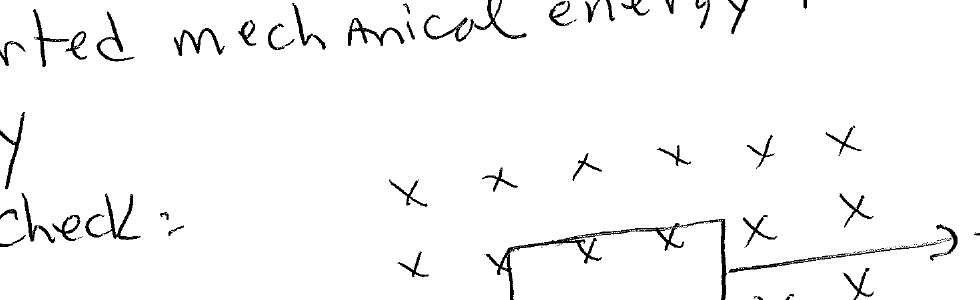
\includegraphics[width=0.55\textwidth,keepaspectratio]{figures/inline/u9_concept_check_loop.png}
  \caption*{Concept check: a loop entirely inside a uniform B-field, pulled at constant speed.}
\end{figure}


What current is induced in a loop sitting \emph{entirely inside} a uniform B-field while being pulled by $F_h$?

\textbf{Answer:} $i = 0$, because the flux $\Phi_B$ is not changing (the loop's full area is in the field). So
\begin{equation}
\mathcal{E} = -\frac{d\Phi_B}{dt} = 0 \implies \frac{\mathcal{E}}{R} = 0
\end{equation}

\section{Time-Varying B-field}

We previously saw we got an EMF when a loop moved in a constant B-field --- because $\Phi_B$ changed. We can also change a flux $\Phi_B$ by varying the $B$ in $\int \vbf{B} \cdot \nhat \, dA$.

\textbf{Experimentally we find} that an EMF develops when $dB/dt \neq 0$ even when there is no circuit. The EMF is associated with an induced \textbf{E-field}:
\begin{equation}
\boxed{-\frac{d\Phi_B}{dt} = \mathcal{E} = \oint \vbf{E} \cdot d\vbf{\ell}}
\end{equation}

\subsection*{Example: Cylindrical Region of Changing B-field}

\begin{figure}[h]
  \centering
  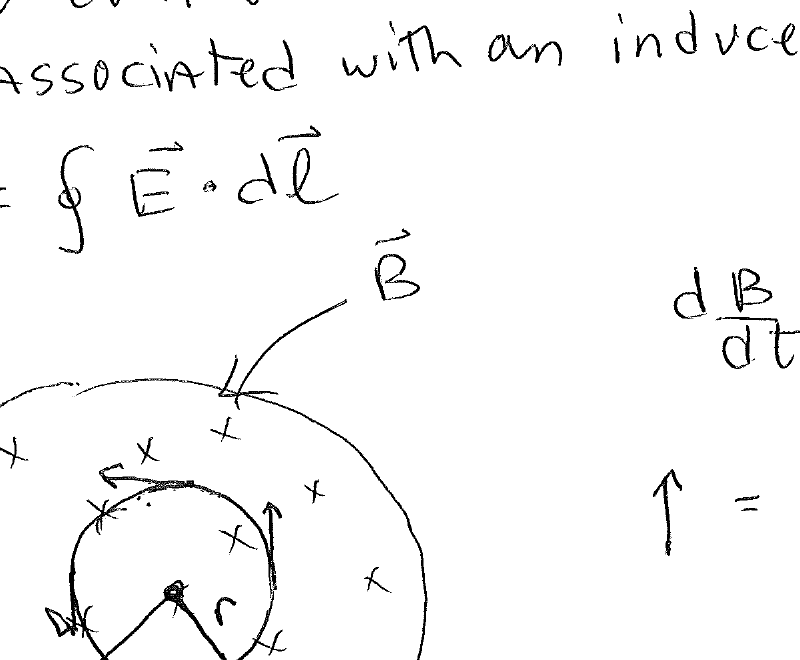
\includegraphics[width=0.5\textwidth,keepaspectratio]{figures/inline/u9_cylindrical_B.png}
  \caption*{Cylindrical region of radius $R$ with a uniform $\vbf{B}$-field out of the page; an increasing $B$ induces a circulating $\vbf{E}$-field.}
\end{figure}


Consider a region $r < R$ where $\vbf{B}$ points into the page and $dB/dt > 0$.

As $dB/dt > 0$, an E-field develops at radius $r$ even though there is no circuit. The direction of $\vbf{E}$ is the same as would be required to drive an induction current at $r$ (by Lenz's Law). The direction of $\vbf{E}$ is determined by symmetry --- it must be tangential and form closed loops.

\subsubsection*{Inside the field region ($r < R$)}

\begin{equation}
\mathcal{E} = -\frac{d\Phi_B}{dt} = -\pi r^2 \frac{dB}{dt}
\end{equation}

If there were an induction current, it would be driven by an $\vbf{E}$ as shown, to oppose the increasing flux in the loop.
\begin{equation}
\mathcal{E} = \oint \vbf{E} \cdot d\vbf{\ell} = E(2\pi r) = -\pi r^2 \frac{dB}{dt}
\end{equation}
\begin{equation}
\boxed{E(r) = -\frac{r}{2} \frac{dB}{dt} \qquad (r < R)}
\end{equation}

This E-field permeates all space at $r < R$.

\subsubsection*{Outside the field region ($r > R$)}

Here the flux is fixed by the field region's area:
\begin{equation}
\Phi_B = \int \vbf{B} \cdot \nhat \, dA = B \pi R^2, \qquad \frac{d\Phi_B}{dt} = \pi R^2 \frac{dB}{dt}
\end{equation}
\begin{equation}
-\mathcal{E} = \oint \vbf{E} \cdot d\vbf{\ell} = E(2\pi r) = \pi R^2 \frac{dB}{dt}
\end{equation}
\begin{equation}
\boxed{E(r) = -\frac{R^2}{2r}\frac{dB}{dt} \qquad (r > R)}
\end{equation}

The field drops like $1/r$ outside the region. (The $-$ sign is just a reminder of Lenz's Law.)

\subsection*{Important Conceptual Point}

\textbf{E-fields generated by time-varying B-fields do NOT have to begin and end on charges. They can form closed loops.}

This is fundamentally different from electrostatics:
\begin{itemize}
    \item \textbf{Electrostatics:} $V_b - V_a = -\int_a^b \vbf{E} \cdot d\vbf{\ell}$, and in a closed loop ($b = a$): $\oint_C \vbf{E} \cdot d\vbf{\ell} = 0$.
    \item \textbf{When $dB/dt \neq 0$:} $\oint_C \vbf{E} \cdot d\vbf{\ell} = -\frac{d\Phi_B}{dt} = -\frac{dB}{dt} A \neq 0$.
\end{itemize}

The induced E-field is non-conservative.

\section{Maxwell's Equations: Getting Close}

We now have three of the four Maxwell equations, plus a near-complete fourth:
\begin{align}
\oint_S \vbf{E} \cdot \nhat \, dA &= \frac{q_{\text{enc}}}{\varepsilon_0} && \text{(Gauss's Law for E)}\\
\oint_S \vbf{B} \cdot \nhat \, dA &= 0 && \text{(Gauss's Law for B)}\\
\oint_C \vbf{E} \cdot d\vbf{\ell} &= -\frac{d}{dt}\int_S \vbf{B} \cdot \nhat \, dA && \text{(Faraday's Law)}\\
\oint_C \vbf{B} \cdot d\vbf{\ell} &= \mu_0 i_{\text{enc}} + (\,?\,) && \text{(Amp\`ere --- something missing!)}
\end{align}

The missing piece in Amp\`ere's Law (the displacement current) will come later --- it is what completes Maxwell's equations and gives rise to electromagnetic waves.

\section{Important Examples}

\subsection{Electric Power Generator}

\begin{figure}[h]
  \centering
  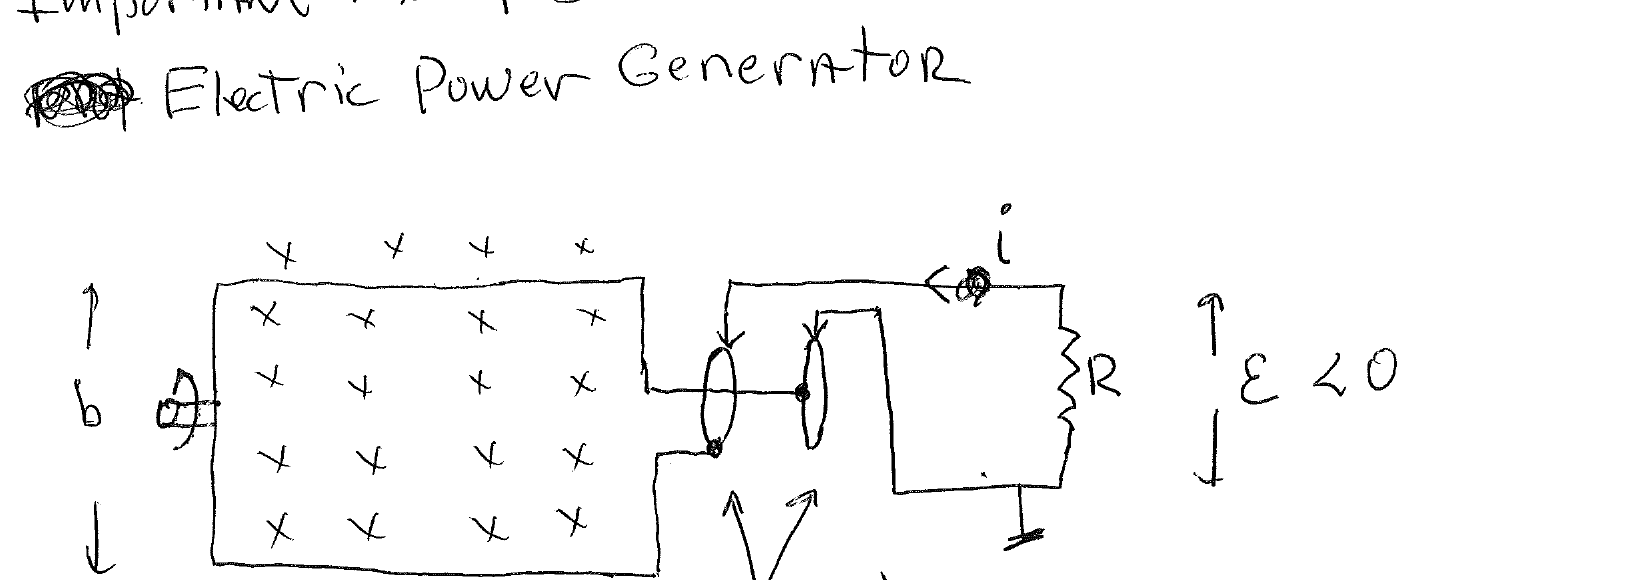
\includegraphics[width=0.85\textwidth,keepaspectratio]{figures/inline/u9_generator.png}
  \caption*{AC generator: a coil of $N$ turns rotates in a uniform B-field; brushes carry the induced EMF to the load $R$.}
\end{figure}


Consider a coil (with $N$ turns, dimensions $a \times b$) rotating at frequency $\nu$ in a uniform magnetic field $\vbf{B}$. The coil is connected via brushes to an external resistor $R$.

The flux is
\begin{equation}
\Phi_B = N\int \vbf{B} \cdot d\vbf{A} = NBab\cos(2\pi\nu t)
\end{equation}

The EMF is, using $\mathcal{E} = -d\Phi_B/dt$:
\begin{equation}
\mathcal{E} = -NBab \cdot \frac{d}{dt}\cos(2\pi\nu t) = NBab(2\pi\nu)\sin(2\pi\nu t)
\end{equation}

So
\begin{equation}
\boxed{\mathcal{E} = \mathcal{E}_0 \sin(2\pi\nu t), \qquad \mathcal{E}_0 = NBab(2\pi\nu)}
\end{equation}
\begin{equation}
i = \mathcal{E}/R
\end{equation}

\subsubsection*{How the brushes work}

As the coil rotates, the current is initially in one direction (e.g., $\mathcal{E} < 0$ relative to ground) because the flux through the coil is decreasing. A half cycle later the flux is increasing and the current must change direction; now $\mathcal{E} > 0$. The brushes have movable contact points to accommodate the changing current direction. (For a DC generator the brushes flip the connection synchronously; for an AC generator they ride on slip rings.)

\subsection{Eddy Currents}

\begin{figure}[h]
  \centering
  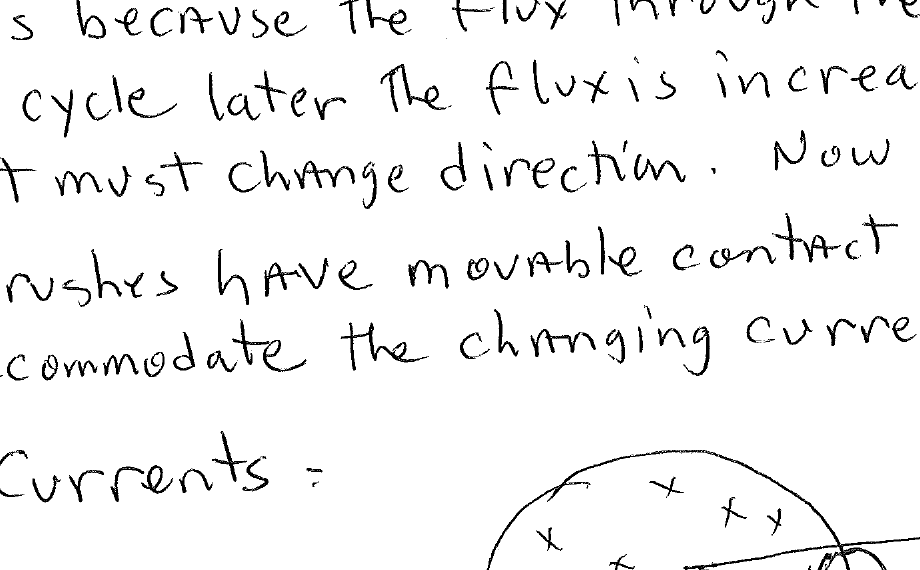
\includegraphics[width=0.55\textwidth,keepaspectratio]{figures/inline/u9_eddy_current.png}
  \caption*{Cu sheet pulled out of a B-field develops a CW eddy current; the $i\vbf{\ell}\times\vbf{B}$ force opposes the motion.}
\end{figure}


Consider a copper sheet being pulled out of a region of B-field (into the page). As the Cu sheet is pulled out, the flux through the Cu sheet decreases.
\begin{enumerate}
    \item A clockwise (CW) eddy current forms whose magnetic dipole is into the page, to oppose the decrease in $\Phi_B$ (by adding B-field to it).
    \item The piece of the eddy current in the B-field has an $i\vbf{\ell}\times\vbf{B}$ that produces a leftward force, opposing the removal of the Cu sheet.
\end{enumerate}

Both are examples of Lenz's Law at work. Eddy currents dissipate energy as heat --- this is the basis of magnetic braking.

\subsection{Electromagnetic Shielding}

\begin{figure}[h]
  \centering
  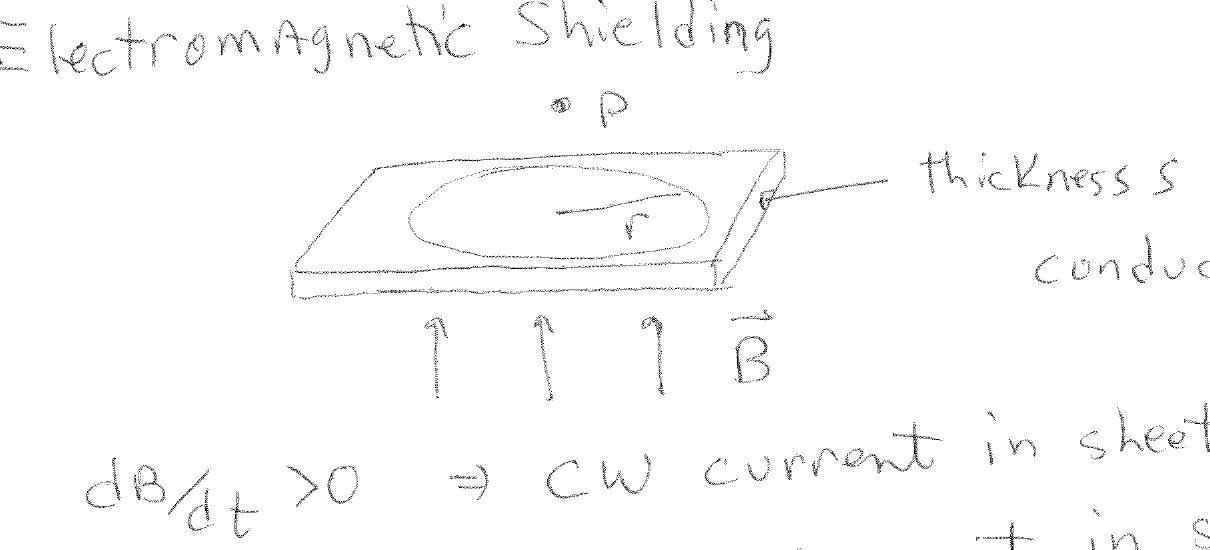
\includegraphics[width=0.7\textwidth,keepaspectratio]{figures/inline/u9_em_shielding.png}
  \caption*{A conducting sheet of thickness $s$ shields point $P$ from a time-varying B-field; induced currents cancel the external flux.}
\end{figure}


Consider a conducting sheet of thickness $s$ and conductivity $\sigma$ above which sits a point $P$. There is an external time-varying B-field $\vbf{B}$ pointing upward, with field changing in time.
\begin{itemize}
    \item $dB/dt > 0 \implies$ CW current in sheet (viewed from above)
    \item $dB/dt < 0 \implies$ CCW current in sheet
\end{itemize}

\subsubsection*{Setting up the calculation}

Consider an Amperian loop of radius $r$ inside the sheet:
\begin{equation}
\mathcal{E} = \frac{d}{dt}\int B\, dA = \pi r^2 \frac{dB}{dt} = \oint \vbf{E} \cdot d\vbf{\ell} = E(2\pi r)
\end{equation}

(The sign is dropped here --- the direction is set by Lenz's Law.)
\begin{equation}
E = \frac{r}{2}\frac{dB}{dt}, \qquad j = \sigma E = \frac{\sigma r}{2}\frac{dB}{dt}
\end{equation}

This is the current density induced in the sheet.

\subsubsection*{Computing the induced current per unit radius}

The induced current is moving in a cross section $dr \times s$:
\begin{equation}
di = j\, dA = j\, s\, dr = \frac{\sigma s}{2} r\, dr \,\frac{dB}{dt}
\end{equation}

\subsubsection*{B-field at the center of an induced ring}

For a current loop, the B-field at the center is $B = \mu_0 i / (2r)$, so each ring contributes
\begin{equation}
dB_0 = \frac{\mu_0 \, di}{2r} = \frac{1}{4}\sigma s \frac{dB}{dt}\mu_0 \, dr
\end{equation}

Integrating from $0$ to $R$ (radius of the induced current region):
\begin{equation}
B_0 = B_{\text{shielding}} = \int dB_0 = \frac{1}{4}\sigma s \mu_0 R \frac{dB}{dt}
\end{equation}

For $dB/dt$ changing rapidly (i.e., high frequency), $B_0$ becomes large and opposes the external $B$, so $B(P) \approx 0$. This is the basis of \textbf{electromagnetic shielding}.

\section{Inductance}

Consider a solenoid carrying current $i$, with a wire loop placed around (or inside) it. The solenoid produces
\begin{equation}
B = \mu_0 n i, \qquad \frac{dB}{dt} = \mu_0 n \frac{di}{dt}
\end{equation}

\textbf{Change current in solenoid $\implies$ change $B$ in loop $\implies$ induced EMF.} This is induction.

\subsection{Self-Induction}

\begin{figure}[h]
  \centering
  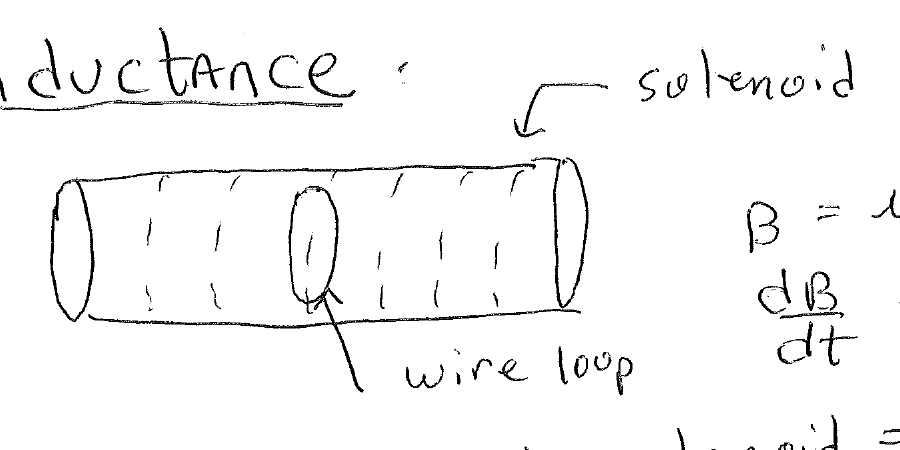
\includegraphics[width=0.55\textwidth,keepaspectratio]{figures/inline/u9_self_induction_solenoid.png}
  \caption*{Solenoid threaded by a wire loop: changing the current in the solenoid induces an EMF in the inner loop.}
\end{figure}


When a current changes in the solenoid, an EMF appears across the solenoid \emph{itself}. This is the \textbf{self-inductance}.

\begin{figure}[h]
  \centering
  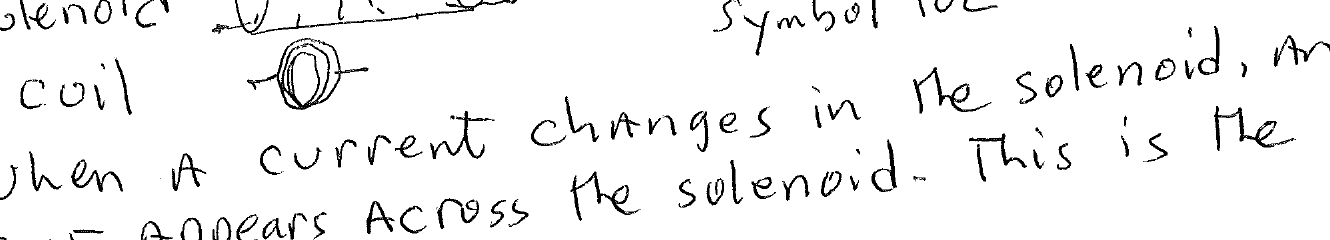
\includegraphics[width=0.6\textwidth,keepaspectratio]{figures/inline/u9_inductor_symbol.png}
  \caption*{Solenoid (or coil) idealized as the circuit symbol for an inductor.}
\end{figure}

\begin{equation}
\mathcal{E} = -\frac{d}{dt}(N\Phi_B), \qquad N\Phi_B = \text{number of flux linkages}
\end{equation}

For a given solenoid (or any shaped coil), the number of flux linkages is proportional to $i$, the current:
\begin{equation}
\boxed{N\Phi_B = Li}
\end{equation}
where $L$, the \textbf{inductance}, is the proportionality constant.
\begin{equation}
\mathcal{E} = -\frac{d}{dt}(N\Phi_B) = -L \frac{di}{dt}
\end{equation}
Or
\begin{equation}
\boxed{L = -\frac{\mathcal{E}}{di/dt}}
\end{equation}

For any geometry --- simple coil, solenoid, toroid --- as long as there is a current, there is a B-field and a self-inductance.

\subsection{Analogy to Capacitance}

\begin{figure}[h]
  \centering
  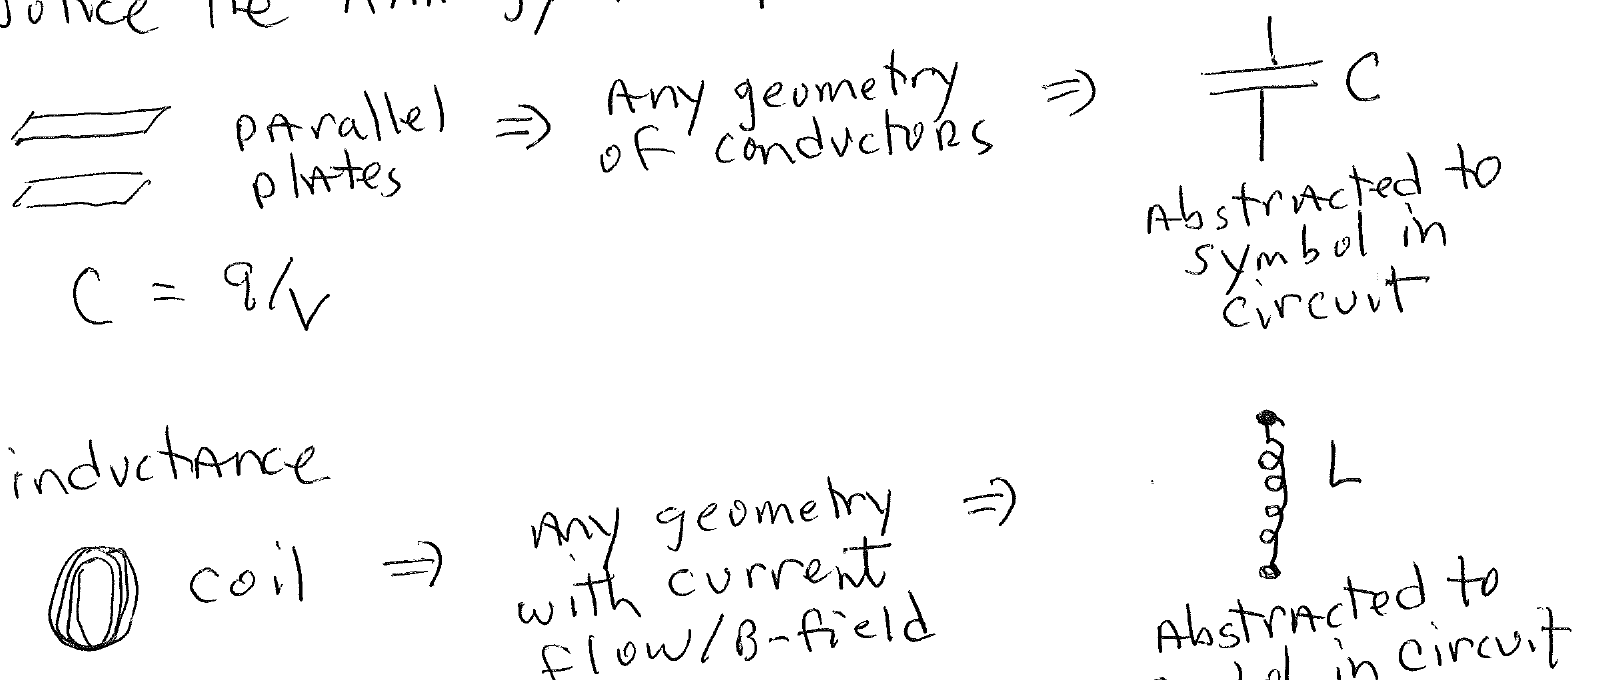
\includegraphics[width=0.85\textwidth,keepaspectratio]{figures/inline/u9_capacitor_inductor_analogy.png}
  \caption*{Analogy: any geometry of conductors yields a capacitance $C$; any geometry with current and a B-field yields a self-inductance $L$.}
\end{figure}


\begin{center}
\begin{tabular}{l|l}
\textbf{Capacitance} & \textbf{Inductance} \\
\hline
Parallel plates $\to$ any geometry of conductors & Coil $\to$ any geometry with current/B-field \\
$C = q/V$ & $L = -\mathcal{E}/(di/dt)$ \\
\end{tabular}
\end{center}

\subsection{Unit of $L$}

\begin{equation}
[L] = \frac{[\text{Volt}]}{[\text{A}/\text{s}]} = \text{Henry (H)}
\end{equation}
\begin{equation}
1\,\frac{\text{Volt}\cdot\text{s}}{\text{A}} = 1\text{ Henry (1 H)} \qquad \text{(SI unit)}
\end{equation}

\section{Calculating Inductance}

\subsection{Solenoid}

\begin{figure}[h]
  \centering
  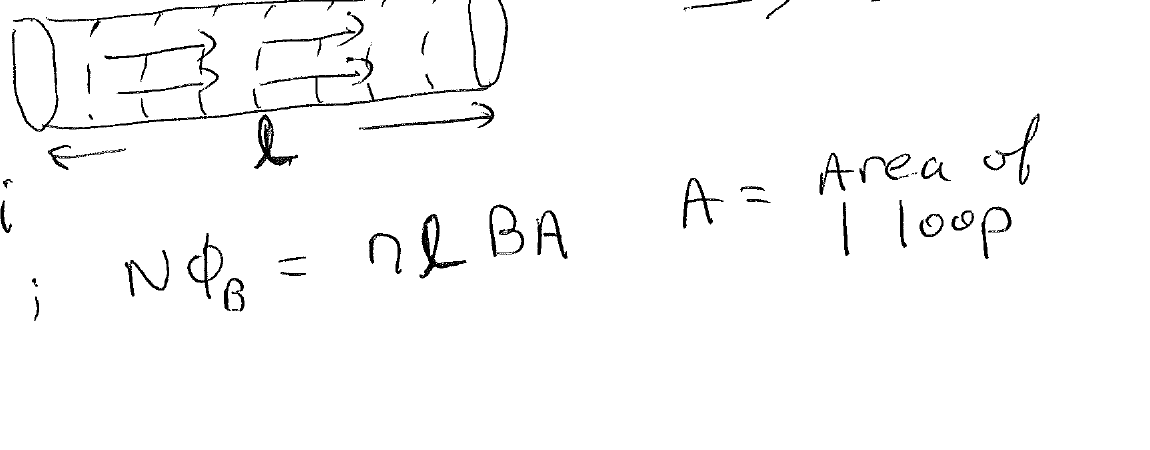
\includegraphics[width=0.55\textwidth,keepaspectratio]{figures/inline/u9_solenoid_geometry.png}
  \caption*{Solenoid of length $\ell$, $n$ turns per unit length, cross-sectional area $A$, carrying current $i$.}
\end{figure}


For a solenoid of length $\ell$, $n$ turns per unit length, cross-sectional area $A$:
\begin{equation}
B = \mu_0 n i, \qquad N = n\ell, \qquad N\Phi_B = n\ell B A
\end{equation}

(Here $A$ = area of one loop.)
\begin{equation}
N\Phi_B = n\ell A (\mu_0 n i) = \mu_0 n^2 \ell A i
\end{equation}
\begin{equation}
\boxed{L = \frac{N\Phi_B}{i} = \mu_0 n^2 \ell A \qquad \text{(inductance of solenoid)}}
\end{equation}

\subsection{Toroid}

\begin{figure}[h]
  \centering
  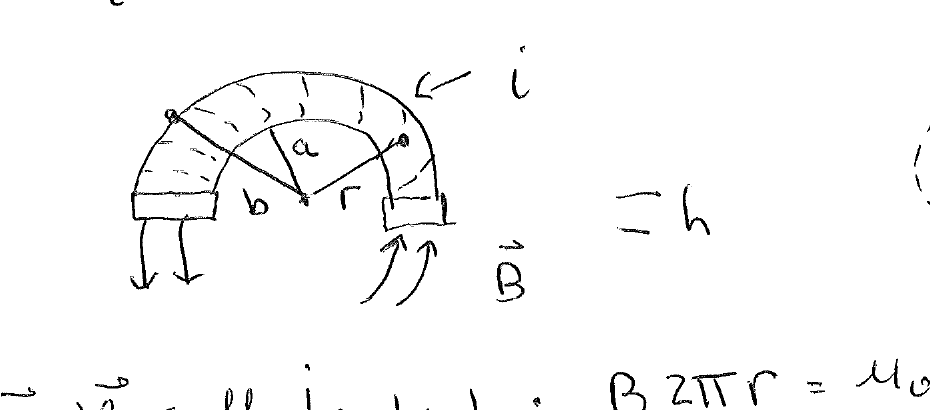
\includegraphics[width=0.55\textwidth,keepaspectratio]{figures/inline/u9_toroid.png}
  \caption*{Toroid of inner radius $a$, outer radius $b$, height $h$, $N$ total turns.}
\end{figure}


A toroid with inner radius $a$, outer radius $b$, height $h$, and $N$ total turns. Use Amp\`ere's Law on a circular Amperian path of radius $r$ inside the toroid:
\begin{equation}
\oint \vbf{B} \cdot d\vbf{\ell} = \mu_0 i_{\text{enc}}, \qquad B(2\pi r) = \mu_0 N i
\end{equation}
\begin{equation}
B(r) = \frac{\mu_0 N i}{2\pi r}
\end{equation}

The flux through one turn (using $dA = h\, dr$):
\begin{equation}
\Phi_B = \int \vbf{B} \cdot d\vbf{A} = \int_a^b \frac{\mu_0 N i}{2\pi r} h \, dr = \frac{\mu_0 N i h}{2\pi}\ln(b/a)
\end{equation}
\begin{equation}
\boxed{L = \frac{N\Phi_B}{i} = \frac{\mu_0 N^2 h}{2\pi}\ln(b/a)}
\end{equation}

\section{LR Circuit}

\begin{figure}[h]
  \centering
  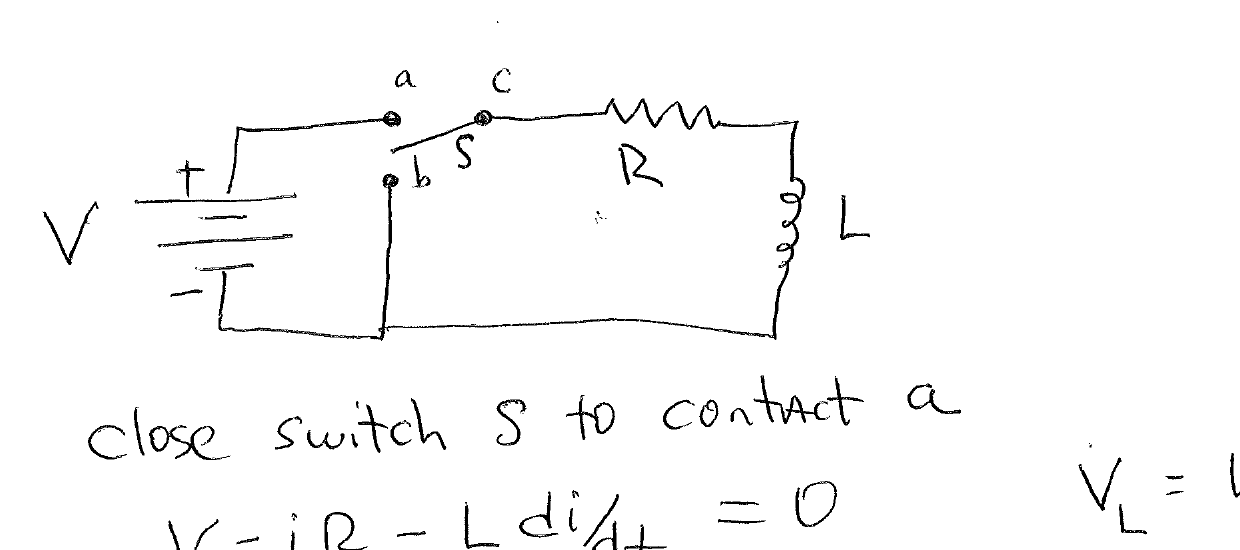
\includegraphics[width=0.7\textwidth,keepaspectratio]{figures/inline/u9_lr_circuit.png}
  \caption*{LR circuit: battery $V$, switch $S$ between contacts $a$ and $b$, resistor $R$, inductor $L$.}
\end{figure}


This is the analog of the RC circuit we studied. Consider a battery $V$, switch $S$, resistor $R$, and inductor $L$ in series. Switch $S$ can be moved to either contact $a$ (charging) or $b$ (discharging).

\subsection{Charging (Switch to $a$)}

Apply Kirchhoff's voltage law:
\begin{equation}
V - iR - L\frac{di}{dt} = 0 \implies \frac{di}{dt} + \frac{i}{(L/R)} = \frac{V}{L}
\end{equation}

(Here $V_L = L\,di/dt$ and $V_R = iR$.) Rewriting,
\begin{equation}
\frac{di}{dt} + \frac{i}{\tau_L} = \frac{V}{L}, \qquad \tau_L \equiv \frac{L}{R} = \text{inductive time constant}
\end{equation}

$L/R$ has units of time (s). The solution is
\begin{equation}
\boxed{i(t) = \frac{V}{R}\left(1 - e^{-t/\tau_L}\right)}
\end{equation}

\begin{figure}[h]
  \centering
  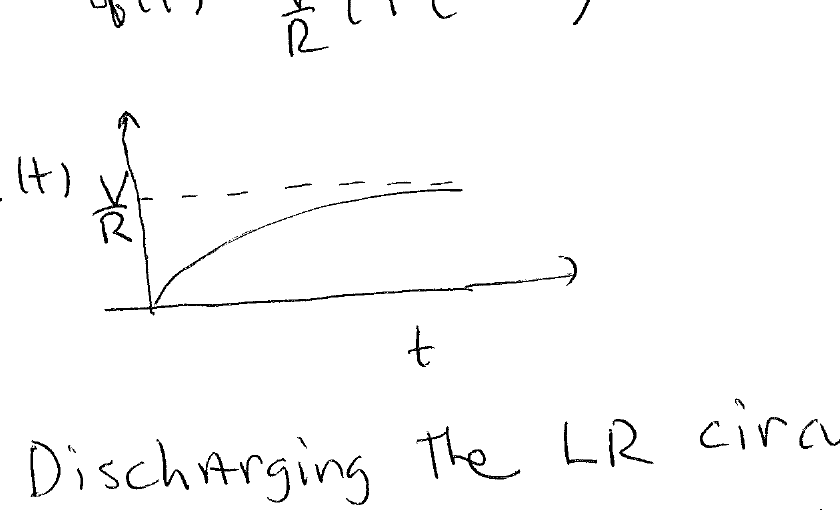
\includegraphics[width=0.45\textwidth,keepaspectratio]{figures/inline/u9_charging_curve.png}
  \caption*{$i(t)$ for the charging LR circuit: rises asymptotically to $V/R$ with time constant $\tau_L = L/R$.}
\end{figure}

In analogy to the RC circuit. The current rises asymptotically to $V/R$ with time constant $\tau_L = L/R$.

\subsection{Discharging the LR Circuit (Switch to $b$ after a long time)}

After a long time, the current is $V/R$. Now move $S$ to $b$ (battery disconnected, loop has only $L$ and $R$):
\begin{equation}
-iR - L\frac{di}{dt} = 0 \implies \frac{di}{dt} + \frac{i}{L/R} = 0
\end{equation}
\begin{equation}
\boxed{i(t) = \frac{V}{R}e^{-t/\tau_L}, \qquad \tau_L = L/R}
\end{equation}

\begin{figure}[h]
  \centering
  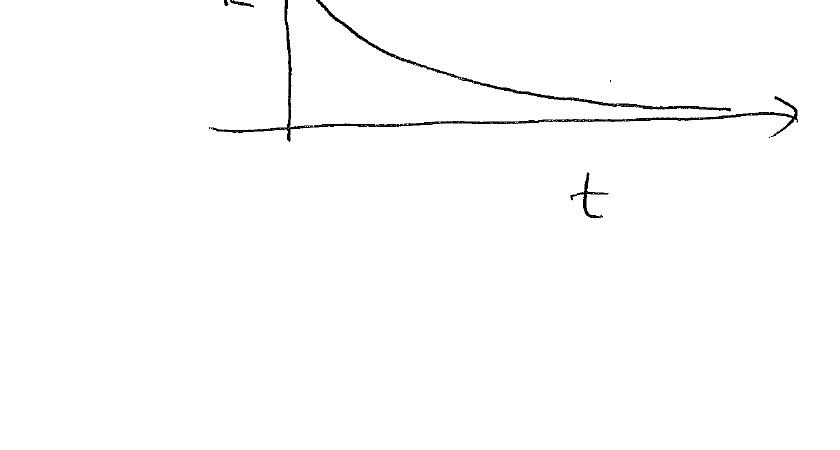
\includegraphics[width=0.45\textwidth,keepaspectratio]{figures/inline/u9_discharging_curve.png}
  \caption*{$i(t)$ for the discharging LR circuit: exponential decay from $V/R$ with the same time constant $\tau_L$.}
\end{figure}

The current decays exponentially.

\subsection{What is going on physically?}

\begin{figure}[h]
  \centering
  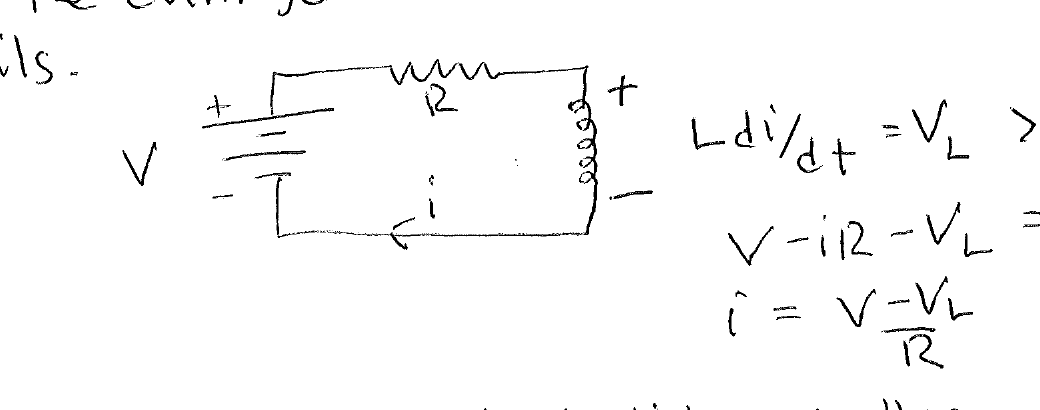
\includegraphics[width=0.65\textwidth,keepaspectratio]{figures/inline/u9_charging_circuit.png}
  \caption*{Charging case: the inductor's induced EMF $V_L$ opposes the increasing current.}
\end{figure}


\textbf{Charging case:} As $i$ increased, the inductor produces an EMF to oppose the change in $i$ and the change in $\Phi_B$ through its coils.

Loop equation:
\begin{equation}
L\frac{di}{dt} = V_L > 0, \qquad V - iR - V_L = 0, \qquad i = \frac{V - V_L}{R}
\end{equation}

But $V_L$ is not constant like a battery --- it depends on $di/dt$. Initially $V_L = V$ (no current can flow yet), and finally $V_L \to 0$ (steady state, current $V/R$).

\textbf{Discharging case:}

\begin{figure}[h]
  \centering
  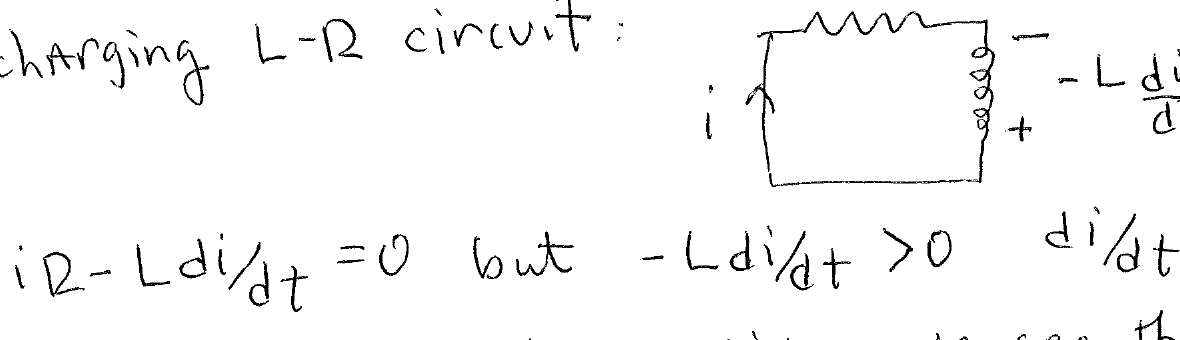
\includegraphics[width=0.55\textwidth,keepaspectratio]{figures/inline/u9_discharging_circuit.png}
  \caption*{Discharging case: with no battery, $-L\,di/dt > 0$ acts to maintain the current as it decays.}
\end{figure}

\begin{equation}
-iR - L\frac{di}{dt} = 0, \qquad \text{but } -L\frac{di}{dt} > 0 \implies \frac{di}{dt} < 0
\end{equation}

So if we define $V_L = -L\,di/dt$, we see that the inductor acts to maintain current in the circuit.

\subsubsection*{Polarity convention}

Some books show the inductor with an EMF arrow:
\begin{itemize}
    \item In the \textbf{charging case}: $\uparrow\mathcal{E}_L$ (EMF produces an E-field to oppose the increase in current)
    \item In the \textbf{discharging case}: $\downarrow\mathcal{E}_L$ (EMF produces an E-field to oppose the decrease in $i$)
\end{itemize}
\begin{equation}
\mathcal{E}_L = L\frac{di}{dt}
\end{equation}

\textbf{The instructor's preferred picture:} Think of it as a potential with the polarities as though a time-dependent battery were acting. In the discharging case the current cannot persist --- it is dissipated in Joule $i^2 R$ loss in the resistor, and in loss of energy stored in the B-field of the inductor.

\section{Energy Stored in an Inductor}

Just as the E-field stores energy in a capacitor, the B-field stores energy in an inductor.

Consider $V = iR + L\,di/dt$. Multiply through by $i$:
\begin{equation}
Vi = i^2 R + Li\frac{di}{dt}
\end{equation}

We know $Vi$ is the power associated with current $i$ driven by potential $V$. $i^2 R$ is the Joule heating loss in resistor $R$. But there is an extra term $L i \, di/dt$. We interpret this as the part of the power going into the inductor --- it is stored there.

The associated energy $U_B$ is obtained as
\begin{equation}
\frac{dU_B}{dt} = Li \frac{di}{dt} \implies \int dU_B = \int Li \frac{di}{dt}\,dt = \int Li \, di
\end{equation}
\begin{equation}
\boxed{U_B = \frac{1}{2}L i^2}
\end{equation}

In analogy to $U_E = \frac{1}{2}q^2/C$.

\section{Energy Density and the B-field}

For a solenoid, the energy is distributed through the volume associated with the B-field, namely $A\ell$. Then the energy density in the B-field is
\begin{equation}
u_B \equiv \frac{U_B}{A\ell} = \frac{\frac{1}{2}Li^2}{A\ell}
\end{equation}

For the solenoid $L = \mu_0 n^2 \ell A$, so
\begin{equation}
u_B = \frac{1}{2}\frac{\mu_0 n^2 \ell A i^2}{\ell A} = \frac{1}{2\mu_0}(\mu_0 n i)^2 = \frac{B^2}{2\mu_0}
\end{equation}
\begin{equation}
\boxed{u_B = \frac{B^2}{2\mu_0}}
\end{equation}

In analogy to the capacitor where $u_E = \frac{1}{2}\varepsilon_0 E^2$.

\section{Coaxial Cable}

\begin{figure}[h]
  \centering
  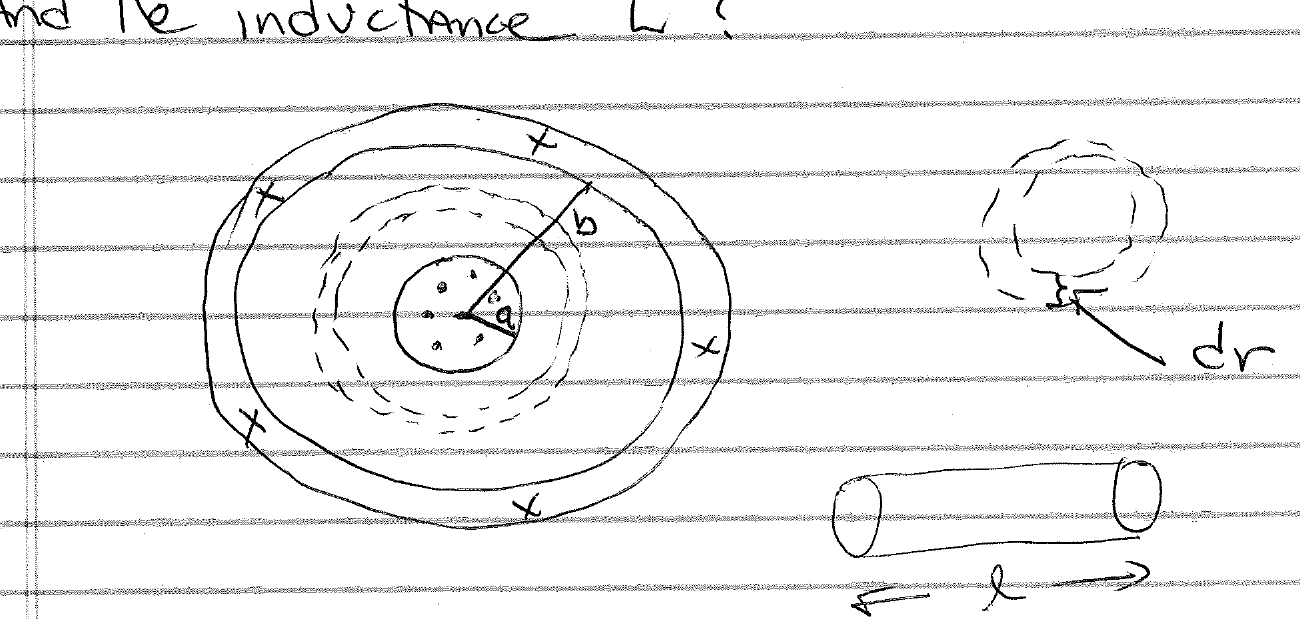
\includegraphics[width=0.7\textwidth,keepaspectratio]{figures/inline/u9_coaxial_cable.png}
  \caption*{Coaxial cable: inner conductor radius $a$ carries current $i$; outer conductor radius $b$ carries return current $i$. The B-field lives in the annulus.}
\end{figure}


Central conductor of radius $a$ carrying current $i$, outer conductor of radius $b$ carrying return current $i$. \emph{What is the energy stored in a cable of length $\ell$, and what is the inductance $L$?}

\subsection*{B-field via Amp\`ere's Law}

At radius $r$ (with $a < r < b$):
\begin{equation}
\oint \vbf{B} \cdot d\vbf{\ell} = \mu_0 i_{\text{enc}} = \mu_0 i \implies B(2\pi r) = \mu_0 i
\end{equation}
\begin{equation}
B(r) = \frac{\mu_0 i}{2\pi r}
\end{equation}

(Not surprising --- this is the same as a long straight wire.)

\subsection*{Energy stored}

Using $u_B = B^2/(2\mu_0)$:
\begin{equation}
U_B = \frac{1}{2\mu_0} \int_V B^2 \, dV
\end{equation}

We need to integrate $B^2$ over the entire volume of the cable. Use cylindrical shells $dV = 2\pi r \, dr \, \ell$:
\begin{equation}
U_B = \frac{1}{2\mu_0} \int_a^b \left(\frac{\mu_0 i}{2\pi r}\right)^2 2\pi r \, dr \, \ell
\end{equation}
\begin{equation}
U_B = \frac{\mu_0 i^2 \ell}{4\pi}\int_a^b \frac{dr}{r}
\end{equation}
\begin{equation}
\boxed{U_B = \frac{\mu_0 i^2 \ell}{4\pi}\ln(b/a)}
\end{equation}

\subsection*{Inductance via energy}

Calculating $U_B$ and getting $L$ from it is often handy because
\begin{equation}
U_B = \frac{1}{2}Li^2 = \frac{\mu_0 i^2 \ell}{4\pi}\ln(b/a)
\end{equation}
\begin{equation}
\boxed{L = \frac{\mu_0 \ell}{2\pi}\ln(b/a)}
\end{equation}

This is the inductance of a coaxial cable of length $\ell$.


\newpage
%==============================================================
% Unit 10: Electromagnetic Oscillations
%==============================================================
\chapter{Electromagnetic Oscillations}

\section{LC Oscillators}

\subsection{Quantitative Analysis}

Consider an ideal LC circuit: an inductor $L$ in series with a capacitor $C$ (no resistance). The total energy in the circuit is
\begin{equation}
E = \underbrace{\tfrac{1}{2}Li^2}_{\text{energy in B-field}} + \underbrace{\frac{q^2}{2C}}_{\text{energy in E-field}}
\end{equation}

Since there is no resistance, energy is conserved:
\begin{equation}
\frac{dE}{dt} = 0 = Li\frac{di}{dt} + \frac{q}{C}\frac{dq}{dt}
\end{equation}

Using $i = dq/dt$ and $di/dt = d^2q/dt^2$:
\begin{equation}
L\frac{dq}{dt}\frac{d^2q}{dt^2} + \frac{q}{C}\frac{dq}{dt} = 0
\end{equation}

Dividing by $L\,dq/dt$:
\begin{equation}
\boxed{\frac{d^2q}{dt^2} + \frac{q}{LC} = 0 \qquad \text{i.e.} \qquad \ddot{q} = -\frac{1}{LC}q}
\end{equation}

\subsection{Analogy to the Simple Harmonic Oscillator}

The equation of motion of a simple harmonic oscillator (mass on a spring) is
\begin{equation}
\ddot{x} = -\frac{k}{m}x
\end{equation}

These are mathematically the \emph{same equation}. Recall the solution to the SHO is
\begin{equation}
x(t) = x_0 \cos(\omega t + \phi), \qquad \omega^2 = \frac{k}{m}
\end{equation}

So the solution to $\ddot{q} = -\frac{1}{LC}q$ is
\begin{equation}
\boxed{q(t) = q_0\cos(\omega t + \phi), \qquad \omega^2 = \frac{1}{LC}}
\end{equation}

The LC circuit oscillates with natural frequency
\begin{equation}
\boxed{\nu = \frac{1}{2\pi\sqrt{LC}}, \qquad \omega = 2\pi\nu}
\end{equation}

\subsection{Setting the Phase from Initial Conditions}

$\phi$ is set by the initial conditions. If at $t=0$, $q = q_0$ (i.e., the capacitor is fully charged and $i = 0$), then $\phi = 0$:
\begin{align}
q &= q_0\cos\omega t = q_0 \quad (t=0) \\
i &= \frac{dq}{dt} = -\omega q_0 \sin\omega t = 0 \quad (t=0)
\end{align}

\subsection{Energy of the Oscillator}

The total energy is $E = U_B + U_E$:
\begin{align}
U_B &= \tfrac{1}{2}Li^2 = \tfrac{1}{2}L\dot{q}^2 = \tfrac{1}{2}L q_0^2 \omega^2 \sin^2\omega t \\
U_E &= \frac{q^2}{2C} = \frac{q_0^2}{2C}\cos^2\omega t
\end{align}

Note that $\tfrac{1}{2}L\omega^2 q_0^2 \sin^2\omega t = \frac{q_0^2}{2C}\sin^2\omega t$ since $\omega^2 = 1/LC$. Therefore:
\begin{align}
E &= \tfrac{1}{2}L\omega^2 q_0^2\sin^2\omega t + \frac{q_0^2}{2C}\cos^2\omega t \\
  &= \frac{q_0^2}{2C}\sin^2\omega t + \frac{q_0^2}{2C}\cos^2\omega t \\
  &= \frac{q_0^2}{2C}
\end{align}

So the total energy is constant:
\begin{equation}
\boxed{E = \frac{1}{2}\frac{q_0^2}{C} = \frac{1}{2}CV_{\max}^2}
\end{equation}
where we used $q_0/C = V_{\max}$. The energy continually sloshes between the capacitor's E-field and the inductor's B-field, but the sum is fixed.

\subsection*{Stages of an LC Cycle (Conceptual Picture)}

In an LC oscillation, the energy moves through eight characteristic stages in each full cycle (analogous to the 8 stages of a mass-on-spring):
\begin{itemize}[leftmargin=*]
    \item \textbf{(a)} Capacitor fully charged, $i = 0$, all energy in E-field.
    \item \textbf{(b)} Capacitor discharging, current building, energy splitting between E-field and B-field.
    \item \textbf{(c)} Capacitor fully discharged, current at maximum, all energy in B-field.
    \item \textbf{(d)} Current still flowing in same direction, charging the capacitor with opposite polarity.
    \item \textbf{(e)} Capacitor fully charged with reversed polarity, $i = 0$, all energy in E-field.
    \item \textbf{(f)--(h)} The cycle proceeds in reverse, returning to (a).
\end{itemize}
The bar graphs of $U_B$ and $U_E$ trade height back and forth, and their sum is constant.

\subsection{Worked Example: Oscillating LC circuit, $L = 10\text{ mH}$, $C = 1\,\mu\text{F}$}

\textbf{(a) What is the frequency of oscillation?}
\begin{equation}
\omega = \frac{1}{\sqrt{LC}} = \left[\frac{1}{(10\times 10^{-3}\text{ H})(1\times 10^{-6}\text{ F})}\right]^{1/2} = 10^4\text{ rad/s}
\end{equation}
\begin{equation}
\nu = \frac{\omega}{2\pi} = 1.6\times 10^3\text{ cycles/s} = 1600\text{ Hz}
\end{equation}

\textbf{(b) If the maximum voltage on the capacitor is 100 V, calculate the maximum current in the inductor.}

From $q = q_0\cos\omega t$ we get $dq/dt = i = -\omega q_0\sin\omega t$, so $i_{\max} = \omega q_0$. Using $q_0 = CV_{\max}$:
\begin{equation}
i_{\max} = \omega C V_{\max} = (10^4\text{ rad/s})(10^{-6}\text{ F})(100\text{ V}) = 1\text{ A}
\end{equation}

\section{Induced B-fields}

\textbf{Experimentally we observe that a changing E-field produces a B-field}, just as a changing B-field produces an E-field.

\subsection*{Setup: Capacitor with Variable Voltage}

Consider a parallel-plate capacitor connected to a battery whose voltage $V$ is being increased ($dE/dt > 0$). Steady current must flow to charge the $+$ plate and push $+$ charge off the $-$ plate. \textbf{Experiment shows that a B-field is then set up} between the plates --- even though no charges are moving across the gap.

\subsection*{Symmetry Picture (View from above the $+$ plate)}

If we view from above, with $\vbf{E}$ pointing into the page (using $\times$ symbols) and increasing in time, the induced $\vbf{B}$-field forms closed loops in the plane of the figure, just as the induced E-field did when $dB/dt \neq 0$.

\textbf{Note the symmetry with the case of $\vbf{E}$ and $\vbf{B}$ reversed.} However:

\textbf{Big difference:} By Lenz's Law, the induced $\vbf{E}$ would be CCW if the $\times$ were $\vbf{B}$. \emph{But in the reverse case where $\times$ is $\vbf{E}$, the induced $\vbf{B}$ is CW.} (The signs in the two laws turn out to be opposite. ``Such is nature.'')

\subsection{Toward Maxwell's Fourth Equation}

We had Faraday's Law:
\begin{equation}
\oint_C \vbf{E}\cdot d\vbf{\ell} = -\frac{d\Phi_B}{dt}
\end{equation}

By analogy, we expect
\begin{equation}
\oint_C \vbf{B}\cdot d\vbf{\ell} = \alpha\,\frac{d\Phi_E}{dt}
\end{equation}
where $\alpha$ is some constant to get the dimensions correct.

\subsection*{Dimensional Analysis to Find $\alpha$}

Take the ratio of the two laws:
\begin{equation}
\frac{\oint \vbf{E}\cdot d\vbf{\ell}}{\oint \vbf{B}\cdot d\vbf{\ell}} \sim \frac{d\Phi_B/dt}{\alpha\, d\Phi_E/dt} \quad \Longrightarrow \quad \frac{E\ell}{B\ell} \sim \frac{BA/t}{\alpha\, EA/t}
\end{equation}
\begin{equation}
\implies \left(\frac{E}{B}\right)^2 = \frac{1}{\alpha}
\end{equation}

Now use $E \sim F/q$ and $B \sim F/(i\ell)$:
\begin{equation}
\left(\frac{E}{B}\right)^2 \sim \frac{(F/q)^2}{(F/i\ell)^2} = \frac{i^2 \ell^2}{q^2} \sim \frac{q^2 \ell^2}{t^2 q^2} = \frac{\ell^2}{t^2}
\end{equation}

So
\begin{equation}
\alpha \sim \left(\frac{\ell^2}{t^2}\right)^{-1} \sim \frac{1}{v^2}
\end{equation}

i.e., $\alpha$ has the dimensions of inverse velocity squared. \textbf{The natural value of $\alpha$ is $\mu_0\varepsilon_0$}, because this combination has SI units of $1/(\text{m}^2/\text{s}^2)$. Therefore:
\begin{equation}
\boxed{\oint_C\vbf{E}\cdot d\vbf{\ell} = -\frac{d\Phi_B}{dt}, \qquad \oint_C\vbf{B}\cdot d\vbf{\ell} = \mu_0\varepsilon_0\,\frac{d\Phi_E}{dt}}
\end{equation}

\subsection*{Speed of Light Emerges}

We are clearly on to something profound, because
\begin{equation}
\frac{1}{\sqrt{\mu_0\varepsilon_0}} = \left[\frac{1}{(4\pi\times 10^{-7})(8.85\times 10^{-12})}\right]^{1/2} = 3\times 10^8\text{ m/s}
\end{equation}

The speed of light is $c = 3\times 10^8$ m/s, so
\begin{equation}
\boxed{c = \frac{1}{\sqrt{\mu_0\varepsilon_0}}}
\end{equation}

We have connected the speed of light to quantities purely associated with E-fields and B-fields. This is the foundation of electromagnetic waves.

\section{Displacement Current}

We had Amp\`ere's Law for magnetostatics:
\begin{equation}
\oint_C \vbf{B}\cdot d\vbf{\ell} = \mu_0 i
\end{equation}

To generalize, we can consider $\oint \vbf{B}\cdot d\vbf{\ell}$ arising from \emph{either} currents $i$ \emph{or} E-field variation $d\Phi_E/dt$. We can generalize Amp\`ere's Law by defining the \textbf{displacement current}:
\begin{equation}
\boxed{i_d \equiv \varepsilon_0\,\frac{d\Phi_E}{dt}}
\end{equation}
so that
\begin{equation}
\boxed{\oint_C \vbf{B}\cdot d\vbf{\ell} = \mu_0(i + i_d) = \mu_0 i + \mu_0\varepsilon_0\,\frac{d\Phi_E}{dt}}
\end{equation}

\subsection*{Why the displacement current matters: continuity of current}

Conduction current $i$ is \emph{not continuous} across the gap in capacitor plates. If we draw a closed path around one wire and use any surface bounded by it, we get different answers depending on whether the surface passes through the wire (which carries current) or threads between the capacitor plates (where no charges flow).

But $dE/dt$ between the plates is exactly what is needed to fix this. With surface charge density $\sigma = q/A$ on the plates:
\begin{equation}
E = \frac{\sigma}{\varepsilon_0} = \frac{q}{\varepsilon_0 A}, \qquad \frac{dE}{dt} = \frac{1}{\varepsilon_0 A}\frac{dq}{dt} = \frac{i}{\varepsilon_0 A}
\end{equation}

Therefore
\begin{equation}
i_d = \varepsilon_0\frac{d\Phi_E}{dt} = \varepsilon_0\frac{d}{dt}(EA) = \varepsilon_0 A\frac{dE}{dt} = i
\end{equation}

\textbf{So the displacement current $i_d$ between the plates equals the conduction current $i$ in the wire.}

\subsection*{The General Picture}

The displacement current gives us a physical picture where there is \emph{continuity of current through the gap}. The conduction current $i$ in the wire becomes a displacement current $i_d$ between the plates, with $i = i_d$.

\section{Maxwell's Equations}

We now have all four:
\begin{align}
\oint_S \vbf{E}\cdot\nhat\, dA &= \frac{q_{\text{enc}}}{\varepsilon_0} && \text{(Gauss's Law for E)} \\
\oint_S \vbf{B}\cdot\nhat\, dA &= 0 && \text{(Gauss's Law for B)} \\
\oint_C \vbf{B}\cdot d\vbf{\ell} &= \mu_0\!\left(i + \varepsilon_0\,\frac{d\Phi_E}{dt}\right) && \text{(Amp\`ere--Maxwell Law)} \\
\oint_C \vbf{E}\cdot d\vbf{\ell} &= -\frac{d\Phi_B}{dt} && \text{(Faraday's Law)}
\end{align}

\textbf{This is a complete classical description of electromagnetism.} Together with the Lorentz force law $\vbf{F} = q\vbf{E} + q\vbf{v}\times\vbf{B}$, these equations describe all classical E\&M phenomena --- including the existence and propagation of electromagnetic waves at speed $c = 1/\sqrt{\mu_0\varepsilon_0}$.


\newpage
%==============================================================
% Unit 11: Electromagnetic Waves
%==============================================================
\chapter{Electromagnetic Waves}

\section{Fields from Time-Varying Sources}

We saw early on that the electric dipole E-field drops like $\propto 1/r^3$, where $r$ is the distance from the dipole. It can also be shown (not done in class but stated in the lecture notes) that the magnetic dipole B-field drops like $\propto 1/r^3$ as well. A more complicated charge distribution drops faster, like $r^{-n}$ (e.g., the quadrupole has $n = 4$).

\textbf{But what if the charges or currents in a distribution vary in time or position?} This is a much more complicated problem than what we have considered so far.

\subsection*{Retarded Fields}

Consider a charge distribution containing many charges, with the $i$th charge at position $\vbf{r}_i$, and a field point $P$:
\begin{equation}
\sum_i \vbf{E}(\vbf{r}_i) = \vbf{E}_P
\end{equation}

The E-field at $P$ from charge $i$ is due to the position of charge $i$ at the \emph{retarded time} $t - |\vbf{r}_i|/c$ --- because electromagnetic information cannot travel faster than the speed of light. So
\begin{equation}
\vbf{E}(\vbf{r}_i) \;\longrightarrow\; \vbf{E}\!\left(\vbf{r}_i,\, t - \frac{|\vbf{r}_i|}{c}\right)
\end{equation}
\begin{equation}
\vbf{E}_P = \sum_i \vbf{E}\!\left(\vbf{r}_i,\, t - \frac{|\vbf{r}_i|}{c}\right)
\end{equation}

So $\vbf{E}_P$ depends on the velocities $\vbf{v}_i$ and on $t$ (through $\vbf{r}_i$). Maxwell's equations still apply, but it takes a lot of work to derive results.

\section{Time-Varying Electric Dipole}

How might we get a time-dependent dipole moment $\vbf{p}(t)$ from our static case? Recall that for two charges $\pm q$ separated by distance $d$ along $\hat{y}$:
\begin{equation}
\vbf{p} = q d \hat{y}
\end{equation}

If we make the charges oscillate up and down, $\vbf{p}$ oscillates in time.

\subsection{LC Oscillator as a Source}

A practical way to make an oscillating dipole is to drive an antenna with an LC oscillator. The setup:
\begin{itemize}
    \item Capacitor $C$ in parallel with inductor $L$ (the primary LC tank).
    \item A second inductor coupled magnetically to $L$.
    \item A transmission line carrying the oscillating current to a dipole antenna.
\end{itemize}

As the LC circuit oscillates, the B-field oscillates and changes direction, so a current is driven in the second inductor by Lenz's Law. Then the antenna develops a potential difference --- effectively, it acts as an oscillating dipole, with charge sloshing back and forth between its two halves.

\subsection{Dipole Radiation}

Since the LC oscillator has $\omega^2 = 1/LC$, the dipole oscillates at this same frequency:
\begin{equation}
\vbf{p}(t) = \vbf{p}_0 \cos\omega t
\end{equation}

The emitted power obeys
\begin{equation}
\frac{dU}{dt} \propto \left(\frac{d^2 \vbf{p}}{dt^2}\right)^2
\end{equation}

Since $d^2\vbf{p}/dt^2 = -\omega^2 \vbf{p}_0 \cos\omega t$, we find
\begin{equation}
\boxed{\frac{dU}{dt} \propto \omega^4}
\end{equation}

This strong frequency dependence is responsible for many phenomena (e.g., why the sky is blue --- Rayleigh scattering goes as $\omega^4$).

\subsection{Polarization of Dipole Radiation}

The dipole antenna produces \textbf{polarized radiation}: the E-field at any field point lies in a specific (fixed) direction set by the orientation of the antenna, and the B-field is perpendicular to it. The radiation propagates in the direction $\vbf{E}\times\vbf{B}$ with $\vbf{E}\perp\vbf{B}$.

\section{Traveling Waves}

We will see that Maxwell's equations in vacuum admit solutions which travel at speed $c$ and oscillate in amplitude. We need a mathematical representation of such waves.

\subsection*{Making a Disturbance Move}

Suppose I have a function $E(x)$ representing the amplitude of an E-field along $\hat{x}$, with peak $E(0) \equiv E_0$ at the origin. I want this ``disturbance'' to move at speed $v$ to the right. What function does this?

If the disturbance moves at speed $v$ and started at $x = 0$, it will be at position $x_0 = vt$ at time $t$, where its amplitude must equal $E_0$. The function
\begin{equation}
E(x,t) = E(x - vt)
\end{equation}
does the job, since
\begin{equation}
E(x_0, t) = E(x_0 - vt) = E(0) = E_0
\end{equation}

So any function $f(x)$ becomes a wave traveling to the right at speed $v$ via
\begin{equation}
\boxed{f(x,t) = f(x - vt) \quad \text{(right-moving)}, \qquad f(x,t) = f(x + vt) \quad \text{(left-moving)}}
\end{equation}

\subsection{Periodic Waves}

Suppose
\begin{equation}
E(x) = E_0 \sin\frac{2\pi x}{\lambda}
\end{equation}
where $\lambda$ is the distance between wave peaks (the \emph{wavelength}) and $E_0$ is the amplitude. Make this a traveling wave by replacing $x \to x - vt$:
\begin{equation}
E(x,t) = E_0 \sin\!\left[\frac{2\pi}{\lambda}(x - vt)\right]
\end{equation}

Define
\begin{align}
k &\equiv \frac{2\pi}{\lambda} && \text{``wave number'' or $k$-vector} \\
\omega &\equiv \frac{2\pi v}{\lambda} = 2\pi\nu && \text{angular frequency} \\
\nu &= \text{frequency}, \qquad T = 1/\nu = \text{period}
\end{align}
Then
\begin{equation}
\boxed{E(x,t) = E_0 \sin(kx - \omega t), \qquad \omega = kv \quad \text{(dispersion relation)}}
\end{equation}

If you stand at position $x_0$, this wave passes you and you undergo one full oscillation in time $T$.

\textbf{Note:} The solution $E = E_0\sin(kx - \omega t)$ together with $\omega = kv$ is the solution to a \emph{specific} differential equation --- the classical wave equation, derived in Section~\ref{sec:wave-eq} below.

\section{Properties of EM Radiation}

For an EM wave moving in the $+x$ direction:
\begin{align}
\vbf{E}(x,t) &= \vbf{E}_m \sin(kx - \omega t) \\
\vbf{B}(x,t) &= \vbf{B}_m \sin(kx - \omega t)
\end{align}
with $\vbf{E}\perp\vbf{B}$. This is a \textbf{plane wave}: the amplitude is constant in the $(y,z)$ plane perpendicular to the propagation direction, and varies only with $x$.

A specific orientation:
\begin{align}
\vbf{E} &= E_m \sin(kx - \omega t)\,\hat{z} \\
\vbf{B} &= B_m \sin(kx - \omega t)\,\hat{y}
\end{align}

Key features:
\begin{itemize}
    \item Direction of propagation = direction of $\vbf{E}\times\vbf{B}$
    \item $\vbf{E}\perp\vbf{B}$
    \item Speed $v \equiv c = 3\times 10^8\text{ m/s}$ (speed of light)
\end{itemize}

\subsection*{How Do We Get a Plane Wave?}

Think of a stone thrown into a pond --- a 2-D wave disturbance propagates outward in concentric circles. The wave fronts move out at speed $v$. For $r$ large, the wave front gets flatter and looks (to an observer at position $x_0$) as though its amplitude is constant in the $y$-direction. As $r\to\infty$, $E(y) = $ const for all $y$. This is the plane wave limit.

\section{The Wave Equation}
\label{sec:wave-eq}

We now derive the wave equation directly from Maxwell's equations in vacuum. Consider an EM wave propagating in $+\hat{x}$, with $\vbf{E}$ along one transverse direction and $\vbf{B}$ along the other. We apply Faraday's Law and Ampere--Maxwell's Law to two narrow rectangular Amperian loops in suitable planes.

\subsection*{Path 1: Faraday's Law}

Choose a rectangular path of width $dx$ and height $h$ in a plane containing $\vbf{E}$. Then
\begin{equation}
\oint_1 \vbf{E}\cdot d\vbf{\ell} = -\frac{\partial}{\partial t}\int_{S_1}\vbf{B}\cdot d\vbf{a}
\end{equation}
\begin{equation}
\oint_1 \vbf{E}\cdot d\vbf{\ell} = h E(x+dx) - h E(x) = -\frac{\partial B}{\partial t}\,h\,dx
\end{equation}
Using $E(x+dx) - E(x) = \dfrac{\partial E}{\partial x}\,dx$:
\begin{equation}
\boxed{\frac{\partial E}{\partial x} = -\frac{\partial B}{\partial t}}
\end{equation}

\subsection*{Path 2: Ampere--Maxwell Law}

Choose a rectangular path of width $dx$ and length $L$ in a plane containing $\vbf{B}$ (no enclosed conduction current in vacuum):
\begin{equation}
\oint_2 \vbf{B}\cdot d\vbf{\ell} = \mu_0\varepsilon_0\,\frac{\partial}{\partial t}\int_{S_2}\vbf{E}\cdot d\vbf{a}
\end{equation}
\begin{equation}
B(x)L - B(x+dx)L = \mu_0\varepsilon_0\,\frac{\partial E}{\partial t}\,L\,dx
\end{equation}
\begin{equation}
\boxed{-\frac{\partial B}{\partial x} = \mu_0\varepsilon_0\,\frac{\partial E}{\partial t}}
\end{equation}

\subsection*{Combining: The Wave Equation}

We have
\begin{equation}
\frac{\partial E}{\partial x} = -\frac{\partial B}{\partial t}, \qquad \frac{\partial B}{\partial x} = -\mu_0\varepsilon_0\,\frac{\partial E}{\partial t}
\end{equation}

Differentiate the first with respect to $x$:
\begin{equation}
\frac{\partial^2 E}{\partial x^2} = -\frac{\partial^2 B}{\partial x\,\partial t}
\end{equation}

Differentiate the second with respect to $t$:
\begin{equation}
\frac{\partial^2 B}{\partial t\,\partial x} = -\mu_0\varepsilon_0\,\frac{\partial^2 E}{\partial t^2}
\end{equation}

Combine:
\begin{equation}
\boxed{\frac{\partial^2 E}{\partial x^2} - \mu_0\varepsilon_0\,\frac{\partial^2 E}{\partial t^2} = 0 \quad \text{i.e.} \quad \frac{\partial^2 E}{\partial x^2} - \frac{1}{c^2}\frac{\partial^2 E}{\partial t^2} = 0}
\end{equation}
since $1/c^2 = \mu_0\varepsilon_0$. By differentiating in the same way for $B$ we obtain
\begin{equation}
\boxed{\frac{\partial^2 B}{\partial x^2} - \frac{1}{c^2}\frac{\partial^2 B}{\partial t^2} = 0}
\end{equation}

This is the \textbf{classical wave equation} for 1-D EM radiation. EM waves propagate in vacuum at speed $c$.

\subsection*{Verifying the Solution}

You can easily check by direct differentiation that
\begin{equation}
E = E_m \sin(kx - \omega t), \qquad B = B_m \sin(kx - \omega t)
\end{equation}
solves the wave equation provided the dispersion relation $\omega = kc$ holds. Substituting:
\begin{equation}
-k^2 \sin(kx-\omega t)\,E_m + \frac{\omega^2}{c^2} E_m \sin(kx-\omega t) = 0 \implies \omega = kc
\end{equation}

\subsection*{Relation between $E$ and $B$ Amplitudes}

Since $\partial E/\partial x = -\partial B/\partial t$, plugging in the wave forms gives
\begin{equation}
k E_m \cos(kx-\omega t) = \omega B_m \cos(kx-\omega t) \implies kE = \omega B
\end{equation}
\begin{equation}
\boxed{B = \frac{E}{c}, \qquad B_0 = \frac{E_0}{c}}
\end{equation}
This is the defining relation between the $B$ and $E$ amplitudes in a plane-parallel EM wave.

\section{Poynting Vector: Energy Transport}

EM waves transport energy. The \textbf{Poynting vector} is
\begin{equation}
\boxed{\vbf{S} \equiv \frac{1}{\mu_0}\vbf{E}\times\vbf{B} = \text{energy crossing unit area in unit time due to EM wave}}
\end{equation}

Its magnitude is
\begin{equation}
|\vbf{S}| = \frac{1}{\mu_0}EB = \frac{dU}{dt}\frac{1}{A}
\end{equation}
where $U$ is the energy of the EM wave. Using $1/\mu_0 = c^2\varepsilon_0$ and $B = E/c$:
\begin{equation}
S = \frac{1}{\mu_0}EB = c\varepsilon_0 E^2
\end{equation}

\subsection*{Time Average $\langle S\rangle$}

For a plane wave $E = E_m\sin(kx-\omega t)$:
\begin{equation}
S = c\varepsilon_0 E_m^2 \sin^2(kx-\omega t)
\end{equation}
The time average of $\sin^2$ over one cycle is $1/2$, so
\begin{equation}
\boxed{\langle S\rangle = \tfrac{1}{2}\varepsilon_0 E_m^2 c = c\, u_{E,\max}, \qquad u_{E,\max} = \tfrac{1}{2}\varepsilon_0 E_m^2}
\end{equation}

\subsection*{Derivation of $S$ from Energy Density}

Consider energy passing through a face of area $A$ of a small cube during time $dt$. The energy in the cube is
\begin{equation}
dU = \left(\tfrac{1}{2}\varepsilon_0 E^2 + \frac{B^2}{2\mu_0}\right)\underbrace{A\,c\,dt}_{dV}
\end{equation}
where $A\,c\,dt$ is the volume of the slab of EM field that crosses the face in time $dt$. Then
\begin{equation}
S = \frac{1}{A}\frac{dU}{dt} = \tfrac{1}{2}\varepsilon_0 E^2 + \frac{B^2}{2\mu_0}
\end{equation}
With $B = E/c$ and $1/\mu_0 = \varepsilon_0 c^2$, the two terms are equal, so
\begin{equation}
S = \varepsilon_0 E^2 c, \qquad \langle S\rangle = \tfrac{1}{2}\varepsilon_0 E_m^2 c
\end{equation}
in agreement with the cross-product definition above.

\section{Polarization}

A dipole antenna emits radiation in which $\vbf{E}$ and $\vbf{B}$ have a definite, fixed orientation as the wave propagates. This is called \textbf{polarized radiation}. Lasers also emit polarized radiation.

This is not the case with most natural sources. An ensemble of atoms emits with each atom's dipole moment randomly oriented, so the radiation is \textbf{unpolarized}.

\subsection*{Polarized EM Wave (View Looking into the Wave)}

Suppose the radiation is approaching us. For an EM wave with $\vbf{E}$ at angle $\theta$ from $\hat{x}$ in the $(x,y)$ plane, any angle $\theta$ is acceptable provided $\vbf{E}\times\vbf{B}$ points out of the page (toward us). For example:
\begin{align}
\vbf{E} &= E_m \cos\theta\,\hat{x} + E_m \sin\theta\,\hat{y} \\
\vbf{B} &= -B_m \sin\theta\,\hat{x} + B_m \cos\theta\,\hat{y} \\
\vbf{E}\times\vbf{B} &= E_m B_m\,\hat{z}
\end{align}

\subsection*{Unpolarized EM Wave}

The ensemble of atoms produces a pattern of $\vbf{E}$ at all possible orientations (and $\vbf{B}$ at right angles to each $\vbf{E}$).

\section{Polarizers}

We can convert unpolarized radiation to polarized radiation with a \textbf{polarizer}. Consider a metal wire in an EM wave whose $\vbf{E}$ is parallel or perpendicular to the wire:

\textbf{$\vbf{E}$ parallel to wire:} The E-field induces an oscillating current of electrons in the wire, i.e., the wire acts like a dipole antenna whose re-emitted field \emph{cancels} the incoming $\vbf{E}$ (and the attached $\vbf{B}$). So $E_P = 0$ on the far side of the wire.

\textbf{$\vbf{E}$ perpendicular to wire:} No current can flow along the wire (no component of $\vbf{E}$ along the wire). The EM wave passes through. $E_P = E$.

In reality we need an array of wires with spacing $d \lesssim \lambda$. This acts like a solid sheet of wires and behaves as described.

\subsection*{Polarizer Transmission (Malus's Law)}

Looking down the propagation direction, the polarizer's wires lie along one axis, and only the projection of $\vbf{E}$ \emph{perpendicular} to the wires can pass through. Assume 100\% polarized incoming radiation with $\vbf{E}$ at angle $\theta$ from the transmission axis (perpendicular to the wires):
\begin{equation}
E_\perp = E_m \cos\theta
\end{equation}

The flux scales as $E^2$:
\begin{align}
S_0 &= \text{initial flux} = K E_m^2, \quad K = \text{constant} \\
S_T &= \text{transmitted flux} = K E_m^2 \cos^2\theta = S_0 \cos^2\theta
\end{align}
\begin{equation}
\boxed{S_T = S_0 \cos^2\theta \quad \text{(Malus's Law)}}
\end{equation}

\textbf{Checks:}
\begin{itemize}
    \item $\theta = 0$: $S_T = S_0$ (100\% transmission). \checkmark
    \item $\theta = \pi/2$: $S_T = 0$ (0\% transmission). \checkmark
    \item $\theta = 45^\circ$: $S_T = S_0/2$ (50\% transmission).
\end{itemize}

In each case the new EM wave is polarized orthogonal to the wire plane.

\subsection*{Unpolarized Radiation Through a Polarizer}

For unpolarized incoming light, $\vbf{E}$ has all possible orientations equally. The probability density of finding the angle between $\vbf{E}$ and the transmission axis to be $\theta$ is
\begin{equation}
p(\theta) = \frac{1}{2\pi} \quad \text{(any angle equally likely)}
\end{equation}
For any $\theta$, $S_T(\theta) = S_0 \cos^2\theta$, so the average transmitted flux is
\begin{equation}
\langle S_T(\theta)\rangle_{\text{all angles}} = \int_0^{2\pi} p(\theta) S_T(\theta)\,d\theta = \frac{1}{2\pi}\int_0^{2\pi} S_0 \cos^2\theta\,d\theta
\end{equation}
Using $\int_0^{2\pi}\cos^2\theta\,d\theta = \pi$ (or the reduction formula $\int\cos^n\theta\,d\theta = \frac{n-1}{n}\int\cos^{n-2}\theta\,d\theta$):
\begin{equation}
\boxed{\langle S_T\rangle = \tfrac{1}{2}S_0}
\end{equation}

So 50\% of unpolarized radiation passes through the polarizer, and the transmitted light is now polarized.

\section{Spherical Waves and Huygens' Principle}

EM waves (as described) are \textbf{transverse waves}: amplitude oscillations are perpendicular to the propagation direction.

Plane waves propagate in one direction with amplitude constant in a plane transverse to that direction. But many sources put out \textbf{spherical waves}, which propagate radially.

\subsection*{Huygens' Principle}

Huygens provided a simple way to understand wave propagation. \emph{Every point on a wave front can be considered the source of spherical wavelets}, and each wavelet propagates an equal distance in equal time. The new wave front is the surface tangent to all the wavelets.

\textbf{Plane wave $\to$ plane wave:} Connect tangents to the wavelets emitted from points along a planar wave front; they propagate as a plane wave. (Ignore the backward-traveling wavelet halves --- this is a known shortcoming of the simplest version of the principle, repaired in the full Kirchhoff formulation.)

\textbf{Spherical wave $\to$ spherical wave:} Tangents to wavelets emitted from a spherical wave front trace out a new (larger) spherical wave front.

Huygens' construction underlies the explanations of reflection, refraction, and diffraction in subsequent units. While visual and geometric, this construction accurately describes the 3-D wave solution of the traveling wave equation. It will be useful when we study diffraction and interference.


\newpage
%==============================================================
% Unit 12: Ray Optics / Geometric Optics
%==============================================================
\chapter{Ray Optics (Geometric Optics)}

\section{Rays}

Another representation, very useful in optics, is to consider \textbf{rays} as lines which propagate \emph{perpendicular} to a wave front.

\textbf{Spherical source:} Draw rays radiating outward, each perpendicular to the spherical Huygens wave fronts.

\textbf{Plane waves:} Rays are parallel straight lines perpendicular to the planar wave fronts.

The Huygens construction explains the alteration of the path of light when it changes from one medium to another. The normals to the wave front are called \textbf{rays}, and are used to formulate geometric optics --- often easier to use than wave fronts.

\section{Snell's Law of Refraction}

\textbf{Key:} The speed of light in a medium is $c/n$, where $n$ is the \textbf{index of refraction} of the medium. In vacuum $n \equiv 1$. In air, $n = 1.0003$.

Each Huygens wavelet on the front advances in steps of $\Delta t$, but in medium $n_2$ travels at $v_2 = c/n_2$, while in medium $n_1$ at $v_1 = c/n_1$. Consider a planar wave front incident at angle $\theta_1$ on the interface, with the refracted front at angle $\theta_2$. The geometry of advancing wavelets gives
\begin{equation}
\sin\theta_1 = \frac{v_1 \Delta t}{L} = \frac{c\,\Delta t/n_1}{L}, \qquad \sin\theta_2 = \frac{v_2\Delta t}{L} = \frac{c\,\Delta t/n_2}{L}
\end{equation}
where $L$ is the distance along the interface between the two ends of the wave front. Dividing one by the other:
\begin{equation}
\boxed{n_1 \sin\theta_1 = n_2 \sin\theta_2 \qquad \text{(Snell's Law)}}
\end{equation}

\subsection*{Example: Light into Glass}

Take $n_{\text{glass}} = 1.6$, $n_{\text{air}} = 1$, incident angle $\theta_1 = 45^\circ$:
\begin{equation}
\sin\theta_1 = n_g \sin\theta_2 \implies \sin\theta_2 = \frac{\sin 45^\circ}{1.6} \implies \theta_2 = 26.2^\circ
\end{equation}

\textbf{Rules of thumb:}
\begin{itemize}
    \item For $n_2 > n_1$: light bends \emph{toward} the normal.
    \item For $n_2 < n_1$: light bends \emph{away} from the normal.
\end{itemize}

\section{Total Internal Reflection}

For a light source in medium 1 with $n_1 < n_2$ swapped --- i.e., light traveling from a \emph{denser} medium ($n_1$) to a \emph{less dense} one ($n_2$, with $n_2 < n_1$) --- there is a critical angle $\theta_c$ where the refracted ray grazes the interface ($\theta_2 = 90^\circ$):
\begin{equation}
n_1 \sin\theta_c = n_2 \sin 90^\circ \implies \boxed{\sin\theta_c = \frac{n_2}{n_1}}
\end{equation}

For $\theta_1 > \theta_c$, no light escapes the medium --- it is all reflected back. This is \textbf{total internal reflection}.

\section{Fiber Optics}

A fiber consists of a core of index $n_{\text{core}}$ surrounded by cladding of index $n_{\text{clad}}$, with $n_{\text{core}} > n_{\text{clad}}$. Light enters the end face from air, refracts into the core, and bounces along by total internal reflection at the core/cladding interface.

\textbf{Setup:} Light at angle $\theta_{1c}$ in air enters the core at the end face, refracting to angle $\theta_2$. It then strikes the side wall at angle $90^\circ - \theta_2$ from the normal of the side wall. For total internal reflection at the side, this angle must equal the critical angle, where the refracted ray would graze ($\theta_3 = 90^\circ$ in cladding):
\begin{align}
n_1 \sin\theta_{1c} &= n_2 \sin\theta_2 \\
n_2 \sin(90^\circ - \theta_2) &= n_3 \sin 90^\circ
\end{align}
With $n_1 = 1$ (air), $n_2 = n_{\text{core}}$, $n_3 = n_{\text{clad}}$:
\begin{align}
\sin\theta_{1c} &= n_{\text{core}} \sin\theta_2 \\
n_{\text{core}} \cos\theta_2 &= n_{\text{clad}} \\
\implies n_{\text{core}}\sin\theta_2 &= n_{\text{core}}\sqrt{1 - (n_{\text{clad}}/n_{\text{core}})^2} = \sqrt{n_{\text{core}}^2 - n_{\text{clad}}^2}
\end{align}
\begin{equation}
\boxed{\sin\theta_{1c} = \sqrt{n_{\text{core}}^2 - n_{\text{clad}}^2}}
\end{equation}

\textbf{Telecommunication fiber:} Cladding is pure silica $n = 1.445$; core is silica doped with GeO$_2$, $n = 1.450$.

For $\theta_1 > \theta_{1c}$, light leaks into the cladding. For $\theta_1 < \theta_{1c}$, light is totally internally reflected and propagates with very low loss.

\subsection*{Numerical Aperture}

Define
\begin{equation}
\sin\theta_{1c} \equiv \mathrm{NA} = \text{numerical aperture}
\end{equation}

The cone of acceptance (solid angle) is
\begin{equation}
\Delta\Omega = 2\pi(1 - \cos\theta_{1c}) = 2\pi\left(1 - \sqrt{1 - \mathrm{NA}^2}\right)
\end{equation}
For $\mathrm{NA} \ll 1$:
\begin{equation}
\Delta\Omega \approx \pi\,\mathrm{NA}^2
\end{equation}
For a typical telecom fiber, $\mathrm{NA} = 0.12$, giving $\Delta\Omega = 0.045$ sr.

\section{Flat Mirrors}

Light reflects from a surface with \textbf{angle of incidence equals angle of reflection}.

\textbf{Image construction:} An object $O$ at distance $o$ from the mirror produces a virtual image $I$ at distance $i$ behind the mirror. To the eye, the diverging reflected rays appear to come from a source at $I$.
\begin{itemize}
    \item $O$ = object (emitter)
    \item $I$ = virtual image
    \item $o$ = object--mirror distance, $i$ = image--mirror distance
\end{itemize}
For a flat mirror,
\begin{equation}
\boxed{-i = o \quad (\text{the } - \text{ sign reminds us it is a virtual image})}
\end{equation}

\section{Curved Mirrors (Concave)}

Geometry of a concave mirror with object $O$ on the optic axis, center of curvature $C$, real image $I$, and a single ray reflecting off the mirror at angle $\theta$ from the local normal (which passes through $C$):
\begin{itemize}
    \item $r$ = radius of curvature
    \item $o$ = object distance, $i$ = image distance
    \item Angles $\alpha$ (at $O$), $\beta$ (at $C$), $\gamma$ (at $I$), where $\alpha, \gamma \ll 1$ (paraxial approximation)
\end{itemize}

\subsection*{Derivation}

By the alternate-exterior-angle relations,
\begin{equation}
\gamma = 2\theta + \alpha, \qquad \beta = \alpha + \theta, \qquad 2\beta - \gamma = \alpha
\end{equation}
For small angles, with arc length $s$ from the optic axis to the reflection point:
\begin{equation}
\alpha = s/o, \qquad \beta = s/r, \qquad \gamma = s/i
\end{equation}
Substituting:
\begin{equation}
\frac{2s}{r} - \frac{s}{i} = \frac{s}{o} \implies \boxed{\frac{1}{o} + \frac{1}{i} = \frac{2}{r}}
\end{equation}

\subsection*{Sign Convention (R-side / V-side)}

Define
\begin{itemize}
    \item \textbf{R-side} = side of the mirror real images form on (in front of mirror)
    \item \textbf{V-side} = side of the mirror virtual images form on (behind mirror)
\end{itemize}

Rules (mirrors):
\begin{itemize}
    \item If $I$ is on R-side: $i > 0$
    \item If $I$ is on V-side: $i < 0$
    \item If $C$ is on R-side: $r > 0$ (concave mirror)
    \item If $C$ is on V-side: $r < 0$ (convex mirror)
\end{itemize}

\section{Parallel Rays and the Focal Plane}

Parallel light rays focus in the \textbf{focal plane}.

\textbf{On-axis source (parallel rays along optic axis):} Take $o \to \infty$ in the mirror equation $1/o + 1/i = 2/r$. Then $i = r/2$. Since this is where parallel light focuses, define the \textbf{focal length}:
\begin{equation}
\boxed{f \equiv \frac{r}{2}, \qquad \frac{1}{o} + \frac{1}{i} = \frac{1}{f}}
\end{equation}

\textbf{Off-axis source (parallel rays at an angle):} Light still focuses in the focal plane, but at an off-axis point $F'$ (or $F''$ on the other side). The set of all such off-axis focal points form the \textbf{focal plane} through $F$.

\section{Images and Ray-Tracing Rules}

To find the image of an extended object of height $h$:

\textbf{Three principal rays (for a concave mirror):}
\begin{enumerate}
    \item A ray through $C$ reflects back through $C$ (it hits normal-on).
    \item A ray through $F$ reflects parallel to the optic axis.
    \item A ray parallel to the optic axis reflects through $F$.
\end{enumerate}

The image height $h'$ has the opposite sign from $h$ (image is inverted).

\subsection*{Magnification}

Geometry shows that
\begin{equation}
\boxed{m = -\frac{i}{o} = \frac{h'}{h}}
\end{equation}
The minus sign indicates the image is upside-down from the object.

\section{Convex Mirror}

For a convex mirror, both $I$ and $C$ are on the V-side, so $i < 0$ and $r < 0$.

\subsection*{Worked Example}

Convex mirror with $r = 20$ cm (so $r = -20$ cm by sign convention), object distance $o = 14$ cm. Where is $I$?
\begin{equation}
\frac{1}{o} + \frac{1}{i} = \frac{2}{r} \implies \frac{1}{14\text{ cm}} + \frac{1}{i} = \frac{2}{-20\text{ cm}}
\end{equation}
\begin{equation}
\frac{1}{i} = -\frac{1}{10\text{ cm}} - \frac{1}{14\text{ cm}} \implies i = -5.8\text{ cm}
\end{equation}
Since $i < 0$, the image is on the V-side (virtual image behind the mirror), as expected for a convex mirror.

\section{Sign Rules: Lenses vs Mirrors}

\subsection*{Lenses (Refraction)}

Signs defined by converging/diverging rays at each surface.

\textbf{Object distance $o$:}
\begin{itemize}
    \item $o > 0$: incident rays at the surface are diverging (real object)
    \item $o < 0$: incident rays are converging (virtual object)
\end{itemize}

\textbf{Image distance $i$:}
\begin{itemize}
    \item $i > 0$: refracted rays are converging (real image)
    \item $i < 0$: refracted rays are diverging (virtual image)
\end{itemize}

\textbf{Radius of curvature $R$:}
\begin{itemize}
    \item $R > 0$: surface is convex as seen by the incoming light
    \item $R < 0$: surface is concave as seen by the incoming light
\end{itemize}

\subsection*{Mirrors (Reflection)}

Signs defined by which side real images form on (R/V rule).

\textbf{Object distance $o$:}
\begin{itemize}
    \item $o > 0$: object on R-side (real object; in front of mirror)
    \item $o < 0$: object on V-side (virtual object; behind mirror)
\end{itemize}

\textbf{Image distance $i$:}
\begin{itemize}
    \item $i > 0$: image on R-side (real image; in front)
    \item $i < 0$: image on V-side (virtual image; behind)
\end{itemize}

\textbf{Radius of curvature $R$:}
\begin{itemize}
    \item $R > 0$: center of curvature on R-side (concave mirror)
    \item $R < 0$: center on V-side (convex mirror)
\end{itemize}

\section{Refracting Surface}

Single spherical refracting surface separating medium $n_1$ from medium $n_2$, center of curvature $C$, radius $r$.

\textbf{Sign rules (refracting surface):}
\begin{itemize}
    \item V-side = incident-light side; R-side = side image forms on
    \item $r < 0$ if $C$ is on V-side; $r > 0$ if $C$ on R-side
    \item $i < 0$ if image on V-side; $i > 0$ if image on R-side
\end{itemize}

\subsection*{Derivation}

A ray from object $O$ hits the surface at angle $\theta_1$ from the normal (which passes through $C$), refracts to angle $\theta_2$, and reaches the image $I$. Define angles $\alpha$ at $O$, $\beta$ at $C$, $\gamma$ at $I$. Geometry gives
\begin{equation}
\theta_1 = \alpha + \beta, \qquad \beta = \theta_2 + \gamma
\end{equation}
Snell's law:
\begin{equation}
n_1 \sin\theta_1 = n_2 \sin\theta_2 \implies n_1 \theta_1 = n_2 \theta_2 \quad \text{(small-angle)}
\end{equation}
With small-angle relations $\alpha \approx s/o$, $\beta \approx s/r$, $\gamma \approx s/i$ (where $s$ is the height of the ray hit on the surface),
\begin{equation}
\beta = \frac{n_1\theta_1}{n_2} + \gamma = \frac{n_1}{n_2}(\alpha + \beta) + \gamma
\end{equation}
Substituting $\alpha, \beta, \gamma$ and simplifying:
\begin{equation}
\boxed{\frac{n_1}{o} + \frac{n_2}{i} = \frac{n_2 - n_1}{r}}
\end{equation}

\section{Thin Lens (Two Refracting Surfaces)}

Combining two refracting surfaces (in the thin-lens approximation, lens thickness much less than other distances) takes much more work but yields the \textbf{lensmaker's equation}:
\begin{equation}
\boxed{\frac{1}{o} + \frac{1}{i} = (n - 1)\left(\frac{1}{r'} - \frac{1}{r''}\right)}
\end{equation}
where $r'$ is the radius of the first surface and $r''$ that of the second. Same sign rules for $i$, $r'$, $r''$ as for the single refracting surface above.

In the form $\dfrac{1}{o} + \dfrac{1}{i} = \dfrac{1}{f}$, the focal length is $\dfrac{1}{f} = (n-1)\!\left(\dfrac{1}{r'} - \dfrac{1}{r''}\right)$.

\section{Rules for Making Images with Lenses}

\subsection*{Converging Lens}

$F_1$ = first focal point (on the incident side); $F_2$ = second focal point (on the far side).

\textbf{Three principal rays:}
\begin{enumerate}
    \item Light parallel to the optic axis $\to$ refracts through $F_2$.
    \item Light through the lens center $\to$ undeflected.
    \item Light through $F_1$ $\to$ comes out parallel to the optic axis.
\end{enumerate}

For an object outside the focal length, the converging lens produces a \textbf{real, inverted} image.

\subsection*{Diverging Lens}

Light parallel to the optic axis diverges on a trajectory that, traced backward, appears to come from $F_1$ on the incident side.

The diverging lens always produces a \textbf{virtual, erect} image (for a real object).


\newpage
%==============================================================
% Unit 13: Diffraction and Interference
%==============================================================
\chapter{Diffraction and Interference}

\section{Optical Path Length}

From Huygens' construction, we can define an advance of a wave in time $\Delta t$ such that
\begin{equation}
\lambda = c\,\Delta t \quad \text{in vacuum}
\end{equation}
i.e., the wave front advances by one wavelength in the period $\Delta t = T = \lambda/c$.

\subsection*{Wavelength in a Medium}

In a medium of index of refraction $n$, the wave advances at speed $c/n$. So in the same time $\Delta t$,
\begin{equation}
\lambda_n = \frac{c}{n}\Delta t \implies \frac{\lambda}{\lambda_n} = \frac{c\,\Delta t}{(c/n)\Delta t} = n \implies \boxed{\lambda_n = \frac{\lambda}{n}}
\end{equation}

\textbf{Check that frequency is unchanged.} In vacuum $\lambda\nu = c$. In medium $\lambda_n \nu_n = v = c/n$. Then
\begin{equation}
\frac{\lambda \nu}{\lambda_n \nu_n} = \frac{c}{c/n} = n
\end{equation}
With $\lambda/\lambda_n = n$, we get $\nu/\nu_n = 1$, so $\nu = \nu_n$.

\textbf{So the frequency of a wave is unchanged in a medium, but the wavelength changes.}

\section{Optical Path Length and Phase Shift}

Suppose we have a medium with index $n_1$ and thickness $\ell_1$. The number of wavelengths that fit inside is
\begin{equation}
N_1 = \frac{\ell_1}{\lambda_{n_1}} = \frac{n_1 \ell_1}{\lambda}
\end{equation}
For another medium of index $n_2$ and thickness $\ell_2$:
\begin{equation}
N_2 = \frac{\ell_2}{\lambda_{n_2}} = \frac{n_2 \ell_2}{\lambda}
\end{equation}

\textbf{Define} the \textbf{optical path length}
\begin{equation}
\boxed{\mathrm{OPL} \equiv n\ell}
\end{equation}
and the optical path length difference
\begin{equation}
\boxed{\Delta \equiv (\mathrm{OPL})_1 - (\mathrm{OPL})_2 = n_1\ell_1 - n_2\ell_2}
\end{equation}

If $\Delta = m\lambda$ ($m$ integer), the waves emerge from the two media \textbf{in phase} --- their maxima and minima overlap. The phase shift between the two waves is
\begin{equation}
\boxed{\phi = 2\pi\,\frac{\Delta}{\lambda} = 2\pi\!\left(\frac{n_1\ell_1 - n_2\ell_2}{\lambda}\right) = k\Delta}
\end{equation}

\subsection*{In Phase / Out of Phase}

If wave 1 is described by $E_1 = E_m\sin(kx - \omega t)$ and wave 2 by $E_2 = E_m\sin(kx - \omega t + \phi)$:
\begin{itemize}
    \item If $\phi = 2m\pi$, $m = 0, 1, 2, \ldots$: $\sin(kx-\omega t + 2m\pi) = \sin(kx-\omega t)$. The waves are \textbf{in phase} and $E_1 + E_2 = 2E_m$.
    \item If $\phi = (2m+1)\pi$, equivalently $\phi = 2(m+\tfrac{1}{2})\pi$: $E_1 + E_2 = 0$. The waves are \textbf{out of phase} by $\pi$ (180\textdegree).
\end{itemize}

\section{A Useful Trick: Adding Waves with a Phase Shift}

Let $\langle S\rangle \equiv I$ denote the intensity. From earlier,
\begin{equation}
I = \frac{c}{2}\varepsilon_0 E_m^2
\end{equation}
where $E_m$ is the amplitude maximum of $\vbf{E}$.

\subsection*{Direct Trig Approach}

Consider $E = E_1 + E_2$ where
\begin{equation}
E_1 = E_m\sin(kx - \omega t), \qquad E_2 = E_m\sin(kx - \omega t + \delta)
\end{equation}
Using the sum-to-product identity $\sin A + \sin B = 2\sin\!\left(\tfrac{A+B}{2}\right)\cos\!\left(\tfrac{A-B}{2}\right)$:
\begin{equation}
E = 2 E_m \cos(\delta/2) \sin(kx - \omega t + \delta/2)
\end{equation}
The intensity is
\begin{equation}
I = c\varepsilon_0 \langle E^2\rangle = 4 c\varepsilon_0 E_m^2 \cos^2(\delta/2) \langle \sin^2(kx-\omega t + \delta/2)\rangle
\end{equation}
Using $\langle\sin^2\rangle = 1/2$:
\begin{equation}
\boxed{I = 2 E_m^2 \cos^2(\delta/2) \times c\varepsilon_0/2}
\end{equation}
(where the proportionality constant is absorbed.)

\subsection*{Complex Notation}

We want to consider an imaginary traveling wave
\begin{equation}
E_1 = E_m e^{i(kx-\omega t)}, \qquad E_2 = E_m e^{i(kx-\omega t + \delta)}
\end{equation}
\textbf{Euler's theorem:} $e^{i\theta} = \cos\theta + i\sin\theta$, so $\mathrm{Im}(e^{i\theta}) = \sin\theta$ and $\mathrm{Re}(e^{i\theta}) = \cos\theta$. Our usual real solution is $E_1 = \mathrm{Im}(E_m e^{i(kx-\omega t)})$, etc.

Adding:
\begin{equation}
E = E_1 + E_2 = E_m e^{i(kx-\omega t)}(1 + e^{i\delta})
\end{equation}
Now factor out $e^{i\delta/2}$:
\begin{equation}
1 + e^{i\delta} = e^{i\delta/2}(e^{-i\delta/2} + e^{i\delta/2}) = 2\,e^{i\delta/2}\cos(\delta/2)
\end{equation}
using $\cos\delta = (e^{i\delta} + e^{-i\delta})/2$. So
\begin{equation}
E = 2 E_m \cos(\delta/2)\, e^{i(kx-\omega t + \delta/2)}
\end{equation}
\begin{equation}
\mathrm{Im}\,E = 2E_m \cos(\delta/2) \sin(kx - \omega t + \delta/2) \quad \checkmark
\end{equation}
matching the trig result.

\subsection*{Intensity in Complex Notation}

Look at $|E|^2 = E E^*$:
\begin{equation}
E E^* = 4 E_m^2 \cos^2(\delta/2)
\end{equation}
So we can use complex $E$ provided we replace $\langle E^2\rangle_{\text{real}}$ with $\tfrac{1}{2}EE^* = \tfrac{1}{2}|E|^2$:
\begin{equation}
\boxed{I = \langle S\rangle = \tfrac{1}{2}\varepsilon_0 c\,|E|^2, \qquad \frac{I}{I_0} = \frac{|E|^2}{|E_0|^2}}
\end{equation}
all in complex notation.

\section{Diffraction vs Geometric Optics}

In geometric optics, light moves in a straight path in parallel bundles --- a plane wave is represented by parallel rays.

Look at an ``obstruction'': a hole in a screen, a slit, a lens, a disk, etc. Let $a$ = hole size and $\lambda$ = wavelength.

\textbf{Case $a \gg \lambda$:} Light passes through in parallel rays --- geometric optics applies. The shape of the light beyond is the geometric projection of the hole.

\textbf{Case $a \lesssim \lambda$:} Light spreads out on passing through the hole. \textbf{This is diffraction.}

\textbf{Criteria:}
\begin{equation}
\boxed{\lambda \ll a \implies \text{geometric optics}, \qquad \lambda \gtrsim a \implies \text{diffraction}}
\end{equation}

\subsection*{Why Does Sound Turn Corners?}

Hearing range: $\nu \sim 20\text{ Hz}$ to $15\text{ kHz}$, $v_{\text{sound}} = 330$ m/s, so $\nu\lambda = 330$ m/s. For a doorway of size $a \approx 1.5$ m, set $\lambda = a$:
\begin{equation}
\nu = \frac{v}{a} = \frac{330\text{ m/s}}{1.5\text{ m}} = 220\text{ Hz}
\end{equation}
For $\nu < 220$ Hz, $\lambda > a$, so we get diffraction of sound waves around the doorway. (This is why bass sounds bend around corners while higher frequencies do not.)

\section{Young's Double-Slit Experiment}

Two slits separated by distance $d$ illuminated by light. Note the waves are interfering --- adding or subtracting in space to the right of the slits.

In each slit the wavelets are in phase. It is easier to analyze with plane waves entering the slits, so use a pinhole at $P$ a long way from the slits, or use a lens to collimate. Setup:
\begin{itemize}
    \item Slits spaced $d$ apart
    \item Screen distance $D$
    \item $\lambda \lesssim a$ (slit width) to ensure each slit diffracts (so that the wavelets spread out from each slit and overlap)
\end{itemize}

\subsection*{Path Difference and Phase Difference}

Let $\ell_1$ and $\ell_2$ be the distances from the two slits to a point on the screen at angle $\theta$ from the central axis. For $D$ large and $\theta$ small ($y/D \ll 1$), the rays $\ell_1$ and $\ell_2$ are approximately parallel. Then the path difference is
\begin{equation}
\Delta = \ell_2 - \ell_1 = d\sin\theta
\end{equation}
and the phase difference is
\begin{equation}
\boxed{\phi = k\Delta = \frac{2\pi}{\lambda}d\sin\theta}
\end{equation}
The two wave peaks are shifted in position relative to one another due to the path-length difference.

\subsection*{Intensity Pattern}

Let $\phi = kd\sin\theta$ and write the two waves in complex form:
\begin{equation}
E_1 = E_m e^{i(kx-\omega t)}, \qquad E_2 = E_m e^{i(kx-\omega t + \phi)}
\end{equation}
\begin{equation}
E_1 + E_2 = E_m e^{i(kx-\omega t)}(1 + e^{i\phi}) = 2 E_m \cos(\phi/2)\, e^{i(kx-\omega t + \phi/2)}
\end{equation}
Single-slit intensity:
\begin{equation}
I_0 = K|E_1|^2 = K E_m^2
\end{equation}
Two-slit intensity:
\begin{equation}
I = K|E|^2 = 4 K E_m^2 \cos^2(\phi/2)
\end{equation}
\begin{equation}
\boxed{\frac{I}{I_0} = 4\cos^2\!\left(\frac{kd\sin\theta}{2}\right) = 4\cos^2\!\left(\frac{\pi d \sin\theta}{\lambda}\right)}
\end{equation}

\subsection*{Intensity Maxima}

Maxima occur where $\cos^2(\phi/2)$ has its maxima:
\begin{equation}
\frac{kd\sin\theta_m}{2} = m\pi \implies \frac{1}{2}\cdot\frac{2\pi}{\lambda}d\sin\theta_m = m\pi
\end{equation}
\begin{equation}
\boxed{m\lambda = d\sin\theta_m, \qquad m = 0, 1, 2, \ldots \quad \text{(maxima)}}
\end{equation}
At each $\theta_m$ we see maxima with $I(\theta_m) = 4 I_0$.

\subsection*{Intensity Minima}

Minima occur for $\cos^2(\phi/2) = 0$:
\begin{equation}
\frac{kd\sin\theta_m}{2} = (m + \tfrac{1}{2})\pi
\end{equation}
\begin{equation}
\boxed{(m + \tfrac{1}{2})\lambda = d\sin\theta_m, \qquad m = 0, 1, 2, \ldots \quad \text{(minima)}}
\end{equation}

\subsection*{Distance Between Adjacent Maxima on the Screen}

Let $y_m$ be the position of the $m$th maximum on the screen. Then $\tan\theta_m = y_m/D$, and for small $\theta_m$:
\begin{equation}
m\lambda = d\sin\theta_m \approx d\tan\theta_m = \frac{d y_m}{D}
\end{equation}
\begin{equation}
y_m = \frac{m\lambda D}{d}
\end{equation}
\begin{equation}
\boxed{\Delta y_m = y_{m+1} - y_m = \frac{\lambda D}{d}}
\end{equation}

\section{Diffraction Gratings ($N$ slits)}

Used in spectroscopy. Consider $N$ slits separated by $d$, each emitting a plane wave to a far point $P$ at angle $\theta$. Each slit has phase shift $\phi = kd\sin\theta$ relative to its adjacent neighbor, so the $n$th slit (counted from the central one as $n=0$) has phase $n\phi$ relative to the central slit.

We must add the E-fields of all the slits at $P$, including the phase shifts:
\begin{equation}
E = \sum_{n=0}^{N-1} E_n, \qquad E_n = E_0 e^{i\phi_n}, \qquad \phi_n = n\phi = n k d\sin\theta
\end{equation}
\begin{equation}
E = \sum_{n=0}^{N-1} E_0 e^{in\phi}
\end{equation}
With single-slit intensity $I_0 = K|E_0|^2$, total intensity $I = K|E|^2$.

\subsection*{Geometric Series Trick}

Use $\sum_{n=0}^{N-1} x^n = (1-x^N)/(1-x)$:
\begin{equation}
E = E_0 \sum_{n=0}^{N-1} e^{in\phi} = E_0\,\frac{1 - e^{iN\phi}}{1 - e^{i\phi}}
\end{equation}
Factor $e^{iN\phi/2}$ from numerator and $e^{i\phi/2}$ from denominator:
\begin{equation}
E = E_0\, e^{i(N-1)\phi/2}\,\frac{e^{iN\phi/2} - e^{-iN\phi/2}}{e^{i\phi/2} - e^{-i\phi/2}}
\end{equation}
Using $\sin x = (e^{ix} - e^{-ix})/(2i)$:
\begin{equation}
\boxed{E = E_0\, e^{i(N-1)\phi/2}\,\frac{\sin(N\phi/2)}{\sin(\phi/2)}}
\end{equation}
\begin{equation}
\boxed{|E|^2 = E_0^2 \left(\frac{\sin(N\phi/2)}{\sin(\phi/2)}\right)^2, \qquad \phi = kd\sin\theta}
\end{equation}

\subsection*{Check: $N=2$ Recovers Two-Slit Result}

\begin{equation}
|E|^2 = E_0^2\left(\frac{\sin\phi}{\sin(\phi/2)}\right)^2 = \left(\frac{2\sin(\phi/2)\cos(\phi/2)}{\sin(\phi/2)}\right)^2 E_0^2 = 4E_0^2\cos^2(\phi/2)
\end{equation}
\begin{equation}
\frac{I}{I_0} = 4\cos^2\!\left(\frac{kd\sin\theta}{2}\right) \quad \checkmark
\end{equation}

\subsection*{Maxima of the $N$-slit Pattern}

These occur where $\sin(\phi/2) = 0$ (where the denominator vanishes and L'Hôpital gives a maximum):
\begin{equation}
\frac{\phi}{2} = m\pi \implies \phi_m = 2\pi m, \qquad \phi = 2\pi, 4\pi, 6\pi, \ldots
\end{equation}

\subsection*{Minima of the $N$-slit Pattern}

These occur where $\sin(N\phi/2) = 0$ but $\sin(\phi/2) \neq 0$:
\begin{equation}
\frac{N\phi}{2} = p\pi \implies \phi_p = \frac{2\pi p}{N}, \qquad p = 1, 2, \ldots, N-1, N+1, \ldots
\end{equation}
The values $p = 0, N, 2N, \ldots$ correspond instead to principal maxima.

\subsection*{Secondary Maxima}

These are at $\dfrac{N\phi}{2} = (p + \tfrac{1}{2})\pi$.

\subsection*{Width of a Principal Peak}

The $m$th principal peak is at $\phi = 2\pi m$ (or equivalently $p = mN$ in the minima index). It is bracketed by minima at $p = mN \pm 1$:
\begin{equation}
\Delta\phi = \frac{2\pi(mN+1)}{N} - \frac{2\pi(mN-1)}{N} = \frac{4\pi}{N}
\end{equation}
The half-width is
\begin{equation}
\Delta\phi_{1/2} = \frac{2\pi}{N}
\end{equation}

\subsection*{Spectral Resolution}

To resolve two spectral lines at $\lambda_1$ and $\lambda_2 = \lambda_1 + \Delta\lambda$, they will occur at angular separation $\delta\theta$:
\begin{equation}
m\,\Delta\lambda = d\cos\theta\,\delta\theta \quad \text{(differentiating } m\lambda = d\sin\theta\text{)}
\end{equation}
To resolve them, the angular separation must be of order the line width of the $m$th peak. In $\theta$-space, the half-width condition $(\Delta\phi)_{1/2} = 2\pi/N = kd\cos\theta\,\delta\theta$ gives
\begin{equation}
\delta\theta = \frac{\lambda}{N d\cos\theta}
\end{equation}
So we can resolve two lines of separation
\begin{equation}
m\,\Delta\lambda = d\cos\theta\,\delta\theta = \frac{d\cos\theta\,\lambda}{Nd\cos\theta} = \frac{\lambda}{N}
\end{equation}
\begin{equation}
\boxed{\frac{\lambda}{\Delta\lambda} = mN \quad \text{(resolving power of an $N$-slit grating)}}
\end{equation}
This is useful for resolving close spectral lines as close as $\Delta\lambda = \lambda/(mN)$, limited by the grating line widths.

\subsection*{Peak Brightness Scales as $N^2$}

For $\phi/2 \to m\pi$, both $\sin(N\phi/2)$ and $\sin(\phi/2)$ go to zero, but
\begin{equation}
\sin(N\phi/2) \to N\phi/2, \qquad \sin(\phi/2) \to \phi/2
\end{equation}
so the ratio $\to N$ and $|E|^2 \to N^2 E_0^2$:
\begin{equation}
\boxed{I_{\max} = N^2 I_0 \quad \text{($N$-slit grating)}}
\end{equation}
The peaks are much brighter than for a 2-slit pattern.

\section{Thin Films}

Light from a source $S$ hits the eye after reflecting off both the top and bottom surfaces of a thin film of index $n$ (e.g., oil on water, soap bubble, AR coating). Rays 1 and 2 (top reflection, bottom reflection) interfere; consider near-normal incidence.

\subsection*{Phase Shifts Induced by Reflection}

\textbf{Rule 1:} If light reflects off an interface from medium $n_1$ to medium $n_2$ with $n_2 > n_1$, the reflected light suffers a phase shift of $\pi$ (180\textdegree).

That is, an incident wave $\sin(kx - \omega t)$ becomes $\sin(kx + \omega t + \pi) = -\sin(kx + \omega t)$ on reflection.

\textbf{Rule 2:} If light reflects from an interface with $n_2 < n_1$, there is \emph{no} phase shift.
\begin{equation}
\sin(kx - \omega t) \to \sin(kx + \omega t) \quad (n_2 < n_1)
\end{equation}

\subsection*{Example: Thin Film on Air}

Film of index $n$ and thickness $d$ in air. The beam splits in two:
\begin{itemize}
    \item Ray 1: reflects off top (air $\to$ film, $n > 1$) $\to$ phase shift $\pi$. So $\phi_2 = \pi$. \emph{(Note: this is the ``second'' ray in the lecture's labeling --- reflected at the top.)}
    \item Ray 1 (going through): travels into the film, reflects off bottom (film $\to$ air, $n_2 < n_1$) $\to$ no phase shift. Travels through extra distance $2d$ in the film, picking up phase from the OPL:
\end{itemize}
\begin{equation}
\phi_1 = \frac{2\pi}{\lambda}(\mathrm{OPL}) = \frac{2\pi}{\lambda}(2nd)
\end{equation}
\begin{equation}
\phi_2 = \pi
\end{equation}

\textbf{Constructive interference} ($\phi_1 - \phi_2 = 2m\pi$):
\begin{equation}
\frac{2\pi(2nd)}{\lambda} - \pi = 2m\pi \implies 2nd = \left(m + \tfrac{1}{2}\right)\lambda
\end{equation}
\begin{equation}
\boxed{2nd = \left(m + \tfrac{1}{2}\right)\lambda \quad \text{(constructive)}}
\end{equation}

\textbf{Destructive interference} ($\phi_1 - \phi_2 = (2m+1)\pi$):
\begin{equation}
\frac{2\pi(2nd)}{\lambda} - \pi = (2m+1)\pi \implies 2nd = (m+1)\lambda
\end{equation}
\begin{equation}
\boxed{2nd = (m+1)\lambda \quad \text{(destructive)}, \qquad m = 0, 1, 2, \ldots}
\end{equation}

\subsection*{Worked Example: Oil Slick at a Gas Station}

$n_{\text{oil}} = 1.48$, $n_{\text{air}} = 1$, $n_{\text{water}} = 1.33$. The oil sits on water with air above. At the air/oil top: $n_2 > n_1$, phase shift $\pi$. At the oil/water bottom: $n_2 = 1.33 < 1.48 = n_1$, so no phase shift. So the same as the film-on-air situation:
\begin{equation}
\phi_1 = \frac{2\pi}{\lambda}(2nd), \qquad \phi_2 = \pi, \qquad 2nd = (m + \tfrac{1}{2})\lambda \quad \text{(constructive)}
\end{equation}

For a 1000 \AA{} oil slick on water, the $m=0$ constructive wavelength is
\begin{equation}
\lambda = 4nd = 4(1.48)(1000\,\text{\AA}) = 5920\,\text{\AA} \implies \text{violet light}
\end{equation}

\subsection*{Anti-Reflection (AR) Coatings}

A thin layer of MgF$_2$ ($n = 1.38$) on glass ($n = 1.5$). At both interfaces (air$\to$MgF$_2$ and MgF$_2$$\to$glass), $n_2 > n_1$, so \emph{both} reflections suffer a $\pi$ phase shift. The two $\pi$ shifts cancel, leaving only the OPL contribution:
\begin{equation}
\phi_1 = \frac{2\pi(2nd)}{\lambda} + \pi, \qquad \phi_2 = \pi
\end{equation}
\begin{equation}
\phi_1 - \phi_2 = \frac{2\pi(2nd)}{\lambda}
\end{equation}
For \textbf{destructive} interference of the reflected light (so all light transmits):
\begin{equation}
\frac{2\pi(2nd)}{\lambda} = (2m+1)\pi \implies \boxed{2nd = (m + \tfrac{1}{2})\lambda \quad \text{(destructive, AR)}}
\end{equation}

For an AR coating optimized at $\lambda = 5500$ \AA{} (the peak of white light) with $n = n_{\text{MgF}_2} = 1.38$ and $m = 0$:
\begin{equation}
d = \frac{\lambda}{4n} = \frac{5500\,\text{\AA}}{4 \times 1.38} = 1000\,\text{\AA}
\end{equation}
A 1000 \AA{} MgF$_2$ coating will do the trick.


\newpage
%==============================================================
% Unit 14: Diffraction
%==============================================================
\chapter{Diffraction}

\section{Diffraction from First Principles}

We saw that Huygens tells us to treat the wave front as composed of secondary wavelets. The total $\vbf{E}$-field at a distant point $P$ is the sum of these wavelets, taking account of their phase shifts.

For a slit (or aperture) with source and screen far from the slit, we have \textbf{Fraunhofer diffraction} (the simplest case --- effectively plane waves in and out).

\section{Single-Slit Diffraction}

\textbf{Setup:} Plane waves incident on a single slit of width $a$. Let $x$ run across the slit. A wavelet at position $x$ travels an extra distance $\Delta = x\sin\theta$ to reach $P$ at angle $\theta$, so its phase shift is
\begin{equation}
\phi(x) = k\Delta = kx\sin\theta
\end{equation}

\subsection*{Sum the Wavelets}

\begin{equation}
E_P = A \int_{-a/2}^{a/2} e^{-ikx\sin\theta}\,dx, \qquad A = \text{constant}
\end{equation}
This is just a sum of Huygens wavelets. The plane wave in the slit (for $\phi(x) = 0$, i.e. $\theta = 0$) is just
\begin{equation}
E_0 = A\int_{-a/2}^{a/2}dx = Aa
\end{equation}

Doing the integral:
\begin{equation}
E_P = A\,\frac{e^{-ika\sin\theta/2} - e^{ika\sin\theta/2}}{-ik\sin\theta} = Aa\,\frac{\sin(ka\sin\theta/2)}{(ka\sin\theta/2)}
\end{equation}
Or
\begin{equation}
\boxed{E_P = E_0\,\frac{\sin(ka\sin\theta/2)}{(ka\sin\theta/2)}}
\end{equation}
\begin{equation}
\boxed{\frac{I}{I_0} = \frac{|E_P|^2}{|E_0|^2} = \left(\frac{\sin(ka\sin\theta/2)}{ka\sin\theta/2}\right)^2}
\end{equation}
This is the \textbf{single-slit diffraction pattern}.

\subsection*{Minima of $I(\theta)$}

These occur where $\sin(ka\sin\theta_m/2) = 0$ but the argument is nonzero:
\begin{equation}
\frac{ka\sin\theta_m}{2} = m\pi \implies \boxed{m\lambda = a\sin\theta_m, \qquad m = 1, 2, 3, \ldots \quad \text{(minima)}}
\end{equation}

\subsection*{Maxima of $I(\theta)$}

The first (central) maximum is at $\theta = 0$, where $\dfrac{\sin x}{x} \to 1$ as $x \to 0$. The other maxima are approximately halfway between minima:
\begin{equation}
\frac{ka\sin\theta_m}{2} = (m + \tfrac{1}{2})\pi \implies \boxed{(m + \tfrac{1}{2})\lambda = a\sin\theta_m, \quad m = 1, 2, 3 \quad \text{(maxima besides } \theta = 0\text{)}}
\end{equation}

\subsection*{Decay of Subsequent Maxima}

For large $m$, the subsequent maxima have intensity
\begin{equation}
\frac{I(\theta_m)}{I_0} \approx \frac{1}{(m + \tfrac{1}{2})^2 \pi^2}
\end{equation}
or simply $1/(m+\tfrac{1}{2})^2$ in the lecture's shorthand --- so they die out very quickly.

\section{Two-Slit Pattern with Single-Slit Diffraction Envelope}

We can now revisit the 2-slit case where we have \textbf{interference} (between the 2 slits) \emph{and} \textbf{diffraction} (within each individual slit). The combined intensity is
\begin{equation}
\boxed{\frac{I(\theta)}{I_0} = \left(\frac{\sin(ka\sin\theta/2)}{ka\sin\theta/2}\right)^2 \cos^2\!\left(\frac{kd\sin\theta}{2}\right)}
\end{equation}
where
\begin{itemize}
    \item $d$ = slit separation (sets the interference fringes)
    \item $a$ = slit width (sets the diffraction envelope)
\end{itemize}
The closely spaced cosine fringes are modulated by the broad sinc envelope.

\subsection*{Aside: Diffraction as a Fourier Transform}

We recognize from our 1-slit integral that the diffraction pattern is just the \textbf{Fourier transform of the aperture}.

\section{Angular Resolution for a Circular Aperture}

(This can be a mirror or a lens.)

For a circular aperture of radius $R$:
\begin{equation}
E \propto \iint_{x^2 + y^2 \le R^2} e^{-ik(x\theta_x + y\theta_y)}\,dx\,dy
\end{equation}
where $\sin\theta_x \approx \theta_x$, $\sin\theta_y \approx \theta_y$, and $\theta^2 = \theta_x^2 + \theta_y^2$. This nasty integral can be done and yields
\begin{equation}
\boxed{\frac{I}{I_0} = \left[\frac{2 J_1(kR\theta)}{kR\theta}\right]^2}
\end{equation}
where $J_1$ is the first-order Bessel function. The pattern is the famous \textbf{Airy disk}: a central peak with concentric rings.

The first zero is at
\begin{equation}
\boxed{\theta_m = \frac{1.22\lambda}{D}, \qquad D = 2R = \text{diameter of aperture}}
\end{equation}

\subsection*{Spot Blurring}

A point source $S$ at distance $r$ imaged by a circular aperture (lens or mirror) of diameter $D$ produces a spot blurred to size
\begin{equation}
\Delta s = \frac{1.22\lambda r}{D}
\end{equation}

\subsubsection*{Hubble Mirror}

Built originally for spy satellites: $D = 2.4$ m, $\lambda = 5\times 10^{-7}$ m (green light), low Earth orbit $r = 400$ km $= 4\times 10^5$ m. Then
\begin{equation}
\Delta s = r\,\frac{1.22\lambda}{D} = 0.1\text{ m} = 10\text{ cm}
\end{equation}
In practice, atmospheric blurring degrades this somewhat.

\subsubsection*{MQ-9 Reaper Drone}

$D \approx 0.3$ m, $r \approx 10$ km $= 33{,}000$ ft, $\lambda = 5\times 10^{-7}$ m:
\begin{equation}
\Delta s = 2\text{ cm}
\end{equation}
Operating at $\approx 15{,}000$ ft, $\Delta s \approx 1$ cm --- can recognize people.

\subsection*{Rayleigh Criterion}

If two point sources are within $\theta_1$ of each other, they are just resolvable when the central maximum of one falls on the first zero of the other:
\begin{equation}
\boxed{\theta_R = \frac{1.22\lambda}{D} \quad \text{(Rayleigh criterion)}}
\end{equation}

\section{Michelson Interferometer --- LIGO}

\textbf{Setup:} A laser provides $E_0$ (intensity $I_0$) into a beam splitter. The beam splits, one beam to mirror $M_1$ (along leg of length $L_x$), one to $M_2$ (along leg of length $L_y$). The reflected beams recombine at the beam splitter, with output going to a detector at the ``dark port.''

Define:
\begin{itemize}
    \item $r_1$ = reflection from beam splitter onto leg 1 $\to M_1$
    \item $r_2$ = reflection from beam splitter after the beam reflects off $M_2$
    \item $t$ = transmission through beam splitter; $t_1 = t_2$
\end{itemize}

Assume $r_{M_1} = r_{M_2} = 100\%$. Assume the beam splitter is coated on the front surface with a 50\% reflector. (This is not strictly true for LIGO but gives the right phase shift in this simpler treatment.)

\subsection*{What is $r_1$?}

Going from air to a dielectric ($1 < n$): a phase shift of $\pi$. Write it as $e^{-i\pi}$ in our complex traveling-wave representation:
\begin{equation}
r_1 = \frac{e^{-i\pi}}{\sqrt{2}}, \qquad r_2 = \frac{1}{\sqrt{2}} \quad (n \to 1, \text{ no phase shift})
\end{equation}
\begin{equation}
t_1 = t_2 = \frac{1}{\sqrt{2}} \quad (\text{50\% transmitting})
\end{equation}
Check: $E_{\text{out}} = \tfrac{1}{\sqrt{2}}E_{\text{in}}$, so $I_{\text{out}} = \tfrac{1}{2}KE_{\text{in}}^2 = I_{\text{in}}/2$.

\subsection*{Equal Arms: Dark Spot at Detector}

Both beams pick up a phase shift $\phi$ at reflection from $M_1/M_2$, but the relative shift is 0, so we ignore it. Start with $L_x = L_y$. Let $E_1, E_2$ be the E-fields entering the detector from legs 1, 2:
\begin{align}
E_1 &= t_1 r_1 E_0 = \frac{1}{\sqrt{2}}\cdot\frac{1}{\sqrt{2}}\,e^{-i\pi}\,E_0 = \tfrac{1}{2}e^{-i\pi}E_0 \\
E_2 &= r_2 t_2 E_0 = \tfrac{1}{2}E_0 \\
E_1 + E_2 &= \tfrac{1}{2}E_0 e^{i(kx-\omega t)}\!\left[1 + e^{-i\pi}\right] = 0
\end{align}
\textbf{There is a dark spot at the detector --- no light. It all went back to the laser!}

\subsection*{Unequal Arms}

The phase shift in each leg is
\begin{equation}
\phi_1 = \frac{2\pi}{\lambda}\cdot 2 L_x, \qquad \phi_2 = \frac{2\pi}{\lambda}\cdot 2 L_y
\end{equation}
The factor of 2 is because the light traverses the leg twice (beam splitter $\to M \to$ beam splitter). Now
\begin{equation}
E_1 = \tfrac{1}{2}E_0 e^{-i\pi} e^{i\phi_1}, \qquad E_2 = \tfrac{1}{2}E_0 e^{i\phi_2}
\end{equation}
Using $e^{-i\pi} = -1$:
\begin{equation}
E_1 + E_2 = \tfrac{1}{2}E_0(e^{i\phi_2} - e^{i\phi_1}) = \tfrac{1}{2}E_0\,e^{i(\phi_2 + \phi_1)/2}\!\left[e^{i(\phi_2 - \phi_1)/2} - e^{-i(\phi_2 - \phi_1)/2}\right]
\end{equation}
\begin{equation}
= i E_0\,e^{i(\phi_2 + \phi_1)/2}\sin\!\left(\frac{\phi_2 - \phi_1}{2}\right) = E_0\,e^{i[(\phi_2+\phi_1)/2 + \pi/2]}\sin\!\left(\frac{\Delta\phi}{2}\right)
\end{equation}
using $e^{i\pi/2} = i$. Thus
\begin{equation}
\boxed{\frac{I}{I_0} = \frac{|E|^2}{E_0^2} = \sin^2\!\left(\frac{\Delta\phi}{2}\right), \qquad \Delta\phi = \frac{2\pi}{\lambda}\cdot 2(L_2 - L_1) = \frac{4\pi(L_2 - L_1)}{\lambda}}
\end{equation}

In reality there are 4 extra mirrors in the legs.

\subsection*{Fabry--Perot Cavity}

These mirrors are highly reflecting, so they trap light for $N \approx 300$ round trips. This is called a \textbf{Fabry--Perot etalon}. So in fact the phase shift is
\begin{equation}
\boxed{\Delta\phi = \frac{4\pi}{\lambda}\,N\,(L_2 - L_1), \qquad N \approx 300}
\end{equation}

\section{Gravitational Waves and LIGO}

The merger of two black holes makes a ripple in the fabric of space-time. This ripple is a \textbf{gravitational wave} and obeys a wave equation:
\begin{equation}
\frac{\partial^2 h_{\mu\nu}}{\partial x^2} - \frac{1}{c^2}\frac{\partial^2 h_{\mu\nu}}{\partial t^2} = 0
\end{equation}
Look familiar? $h$ describes the distortion of our rulers in the presence of the GW.

The GW has the property that when it arrives with the proper orientation (polarization!) to the interferometer, it alters lengths in space-time. \textbf{The mirrors don't move --- the rulers change.} Recipe: for $L_x = L_y = L$ before the wave (we'll get the dark spot),
\begin{align}
L_x &= L + \tfrac{h}{2}L = L(1 + h/2) \\
L_y &= L - \tfrac{h}{2}L = L(1 - h/2) \\
L_2 - L_1 &= L + \tfrac{h}{2}L - L + \tfrac{h}{2}L = hL = \Delta L
\end{align}
\begin{equation}
\Delta\phi = \frac{4\pi}{\lambda}\,N\,h L
\end{equation}

\subsection*{LIGO Numbers}

$N \approx 300$, $\lambda = 1.06\,\mu$m (Nd:YAG laser), $L = 4$ km, $h \approx 10^{-21}$ (!).

The relative shift of the mirrors is
\begin{equation}
\Delta L = h L = 10^{-21} \times 4000\text{ m} = 4 \times 10^{-18}\text{ m}
\end{equation}
This is about $\tfrac{1}{1000}$ the diameter of a \textbf{nucleus!}
\begin{equation}
\Delta\phi = 1.4\times 10^{-8}\text{ rad at the detector}
\end{equation}

\subsection*{LIGO Trick}

Detune from $L_1 = L_2$ (the dark spot) by $\delta \approx 10^{-2}$ rad, i.e., $k(L_2 - L_1) = \delta$. Then
\begin{equation}
\frac{I}{I_0} = \sin^2\!\left(\frac{\Delta\phi + \delta}{2}\right) = \tfrac{1}{2}\!\left[1 - \cos(\Delta\phi + \delta)\right]
\end{equation}
Expand using $\cos(\delta + \Delta\phi) = \cos\delta\cos\Delta\phi - \sin\delta\sin\Delta\phi$. With $\cos\Delta\phi \approx 1$, $\sin\Delta\phi \approx \Delta\phi$, $\delta \ll 1$:
\begin{equation}
I = \tfrac{I_0}{2}(1 - \cos\delta) + \tfrac{I_0}{2}\sin\delta \,\Delta\phi
\end{equation}
The first term is constant (DC component); the second is the signal.
\begin{equation}
\Delta I \approx \tfrac{I_0}{2}\delta\,\Delta\phi = \tfrac{I_0}{2}\delta\!\left(\frac{4\pi N hL}{\lambda}\right)
\end{equation}

Now use power: $P_{\text{DC}} \approx P_0\,\delta^2/4$, $\Delta P = P_0\,\delta\,\Delta\phi/2$, so
\begin{equation}
\frac{\Delta P}{P_{\text{DC}}} = \frac{2\Delta\phi}{\delta}
\end{equation}
With $P_0 \approx 100$--$300$ kW, $P_{\text{DC}} \approx 10$--$50$ mW. Plugging in $\delta$, $\Delta\phi$:
\begin{equation}
\Delta P \approx 30\text{--}150\text{ nW} \quad \text{--- this is measurable!}
\end{equation}

\subsection*{Technical Notes}

Strictly, LIGO does not use a front-coated mirror. However when a more detailed analysis of a beam splitter is done, we find we pick up the minus sign --- i.e., $e^{i\phi_1} - e^{i\phi_2}$, just as though we had a relative phase shift of $\pi$ at the beam splitter. The cavity mirrors are also a bit more complicated to treat, but in the end we get the relative phase shift we obtained, with some extra prefactors.

\section{Bragg Diffraction}

An X-ray beam incident on a crystal will diffract with the array of atoms as though they are a 3-D aperture. In fact, the X-rays interact with planes of atoms in the crystal. Each unit cell of the crystal acts as a source of (Huygens) wavelets. It is the X-rays scattering from atomic electrons that produce the diffracted beam.

\subsection*{Bragg's Law}

Consider a crystal lattice with atom spacing $D$ and a particular set of crystal planes separated by $d = D\sin\theta$ where $\theta$ is the angle of incidence measured from the lattice. The scattered angle from the incident direction is $\phi = 2\theta$ (total scatter angle).

Path-length difference between adjacent planes:
\begin{equation}
\Delta = d\cos\theta
\end{equation}
For constructive interference:
\begin{equation}
2\Delta = n\lambda \implies \boxed{2d\cos\theta = n\lambda}
\end{equation}

(Bragg diffraction is usually defined via the angle $\alpha$ measured from the plane: $n\lambda = 2d\sin\alpha$. Here, $\alpha$ is complementary to the lecture's $\theta$.)

But $2d\cos\theta = 2D\sin\theta\cos\theta = D\sin 2\theta$, so
\begin{equation}
\boxed{n\lambda = D\sin\phi, \qquad \phi = \text{total scatter angle}}
\end{equation}

\subsection*{Multiple Plane Families}

There are many planes that will give Bragg peaks on diffraction. The obvious one (horizontal rows with spacing $D$) gives $2D\cos\theta = n\lambda$, with $\theta = \phi/2$, so $2D\cos(\phi/2) = n\lambda$. This produces another set of Bragg peaks.

\subsection*{Example: Nickel Crystal}

For nickel, $D = 2.15$ \AA. For 1.65 \AA{} X-rays incident, the Bragg peak is at $\phi = 50^\circ$.

\section{De Broglie Waves}

De Broglie postulated that to a particle of mass $m$ we should assign a wavelength, the \textbf{de Broglie wavelength}, such that
\begin{equation}
\boxed{\lambda_{\text{dB}} = \frac{h}{p}}
\end{equation}
With $p = mv$ and $E = p^2/(2m)$, so $p = \sqrt{2mE}$. Here $h = 6.6\times 10^{-34}$ J$\cdot$s is \textbf{Planck's constant}.

\subsection*{Davisson--Germer Experiment}

Clinton Davisson and Lester Germer were shooting 54 eV electrons at a nickel film which had been inadvertently crystallized.
\begin{align}
m_e &= 9.1\times 10^{-31}\text{ kg}, \qquad E_e = 8.65\times 10^{-18}\text{ J} \\
h &= 6.6\times 10^{-34}\text{ J$\cdot$s} \\
\lambda_{\text{dB}} &= \frac{h}{\sqrt{2 m_e E}} = 1.65\text{ \AA{}} = 1.65\times 10^{-10}\text{ m}
\end{align}
Shooting these electrons at the nickel they found a Bragg peak at $50^\circ = \phi$!

\textbf{This established the wave nature of particles and thus the wave--particle duality.} Electrons travel as waves but are detected as particles. For this Davisson won the Nobel Prize.

\section{Relation of Classical Wave Equation to Quantum Mechanics}

\subsection*{Classical Wave}

A wave of real amplitude $E$:
\begin{equation}
E = E_0 e^{i(kx-\omega t)} \quad \text{(trick)}
\end{equation}
But in the end we must take
\begin{equation}
\mathrm{Re}\,E = E_0\cos(kx-\omega t) \quad \text{or} \quad \mathrm{Im}\,E = E_0\sin(kx-\omega t)
\end{equation}
These are real things with a real, measurable E-field. The wave equation
\begin{equation}
\frac{\partial^2 E}{\partial x^2} - \frac{1}{c^2}\frac{\partial^2 E}{\partial t^2} = 0
\end{equation}
Plugging in $E = E_0 e^{i(kx-\omega t)}$:
\begin{equation}
\left[-k^2 + \frac{\omega^2}{c^2}\right] E_0 e^{i(kx-\omega t)} = 0 \implies \omega = kc \implies \nu\lambda = c
\end{equation}

\subsection*{Quantum Mechanics: The Schr\"odinger Equation}

To the particle there exists a wave function $\psi$. It obeys a wave equation, the \textbf{Schr\"odinger equation} (for non-relativistic particles). $\psi$ is the wave amplitude. In 1-D (particle moving force-free):
\begin{equation}
\boxed{-\frac{\hbar^2}{2m}\frac{\partial^2 \psi}{\partial x^2} - i\hbar\,\frac{\partial\psi}{\partial t} = 0, \qquad \hbar \equiv \frac{h}{2\pi}}
\end{equation}

Let $\psi = \psi_0 e^{i(kx-\omega t)}$.

\textbf{Note:} $\sin(kx-\omega t)$ and $\cos(kx-\omega t)$ are \emph{not} solutions to this equation. $\psi$ \emph{must} be imaginary (complex) here. (This is fundamentally different from the classical wave equation.)

Plugging in:
\begin{equation}
\left[\frac{\hbar^2 k^2}{2m} - \hbar\omega\right]\psi_0 e^{i(kx-\omega t)} = 0
\end{equation}
\begin{equation}
\hbar\omega = \frac{\hbar^2 k^2}{2m}
\end{equation}
Identify
\begin{equation}
\boxed{E = \hbar\omega = \text{energy of particle}, \qquad p = \hbar k = \text{momentum of particle}}
\end{equation}
Note
\begin{equation}
p = \hbar k = \frac{h}{2\pi}\cdot\frac{2\pi}{\lambda} = \frac{h}{\lambda} \implies \lambda = \frac{h}{p}
\end{equation}
\textbf{The de Broglie wavelength falls right out of the equation!}

\subsection*{Born's Postulate: Probability}

De Broglie guessed at the wave-like nature of particles. Everyone asked: what is the wave equation associated with the wavelength? Schr\"odinger answered.

But we saw a real diffraction pattern from electrons scattering off nickel, and we see it with a 2-slit experiment. But $\psi$ is not real. We saw we get $I/I_0$ in the classical wave equation by $I/I_0 = |E|^2/|E_0|^2$. We saw this was just a trick because $E$ is real. But if we assume physical reality is in
\begin{equation}
\boxed{|\psi|^2 = \psi^*\psi}
\end{equation}
we have a real number, and so
\begin{equation}
\frac{I}{I_0} = \frac{|\psi|^2}{|\psi_0|^2}
\end{equation}
Our previous analysis of 2-slit interference carries through exactly.

\textbf{M. Born won the Nobel Prize for postulating reality is in $|\psi|^2$, not $\psi$.}

For the 2-slit interference experiment, electrons over time will build up the pattern
\begin{equation}
\frac{|\psi(\theta)|^2}{|\psi_0|^2} = \cos^2\!\left(\frac{kd\sin\theta}{2}\right), \qquad k = p/\hbar
\end{equation}
But the electrons approach the screen \emph{individually}. The probability that one lands at $\theta$ is given above. But \textbf{one by one, we cannot predict where it will land}. We have lost the classical determinism of Newtonian physics. We only have probabilistic knowledge of the electron's trajectory after the slit.

We do, however, have a \textbf{quantum determinism} in that the Schr\"odinger equation determines $\psi(x,t)$ for all times, just like $F = ma$ determines particle motion for all time.


\end{document}
